\documentclass[11pt, a4paper]{article}
\usepackage[utf8]{inputenc}

\usepackage{listings}
\usepackage[framed,numbered,autolinebreaks,useliterate]{mcode}

\usepackage[margin=1in]{geometry}
\usepackage{graphicx}
\usepackage{amsmath}
\usepackage{amsfonts}
\usepackage{float}
\graphicspath{ {../images/} }
\setlength\parindent{0pt}


\newcommand{\p}{\partial}
\newcommand{\mth}[1]{
  \begin{align*}
    #1
  \end{align*}
}



\begin{document}

\begin{center}
  \Huge ECEN4532, DSP Laboratory \\
  \huge Audio Analysis \\
  \huge Lab 1\\
  
  \vspace{7in}
    \huge Jeffery Lim \\
    \huge Jeffery.Lim@colorado.edu\\~\\~\\
\end{center}
\pagebreak


\tableofcontents

\pagebreak

\section{Introduction}

For this lab, audio analysis techniques were utilized in order to see how they could provide useful to be able to detect and organize different genres of music. Time domain and spectral analysis both provide to give different information, some more meaningful than others. The first area of interest was in the time domain, where we analyze the loudness of the song for a given frame as well as the zero-crossing rate. The second area of interest is to taking the signal into the Fourier domain and analyze the frequencies of the signal. Each track had its spectrogram, spectral centroid, spread, flatness, and flux analyzed and determined if they were any useful to genre classification. The third and last area of interest is the creation of filter banks to filter the audio signal and to use the cochlear filter banks to produce a mel-spectrum (MFCC) coefficient plot. All the code was written in Matlab and the workspace script can be found in the Appendix.

\subsection{Sampling Frequency (1)}

Since dolphins hear from 7 - 120 KHz, we would require that the sampling frequency, $f_s$ should be at least double the highest frequency required: 240 KHz.

\section{Audio Extracting}

In order to extract audio from a song, the sampling frequency of the audio is required. Knowing the sampling frequency, allows extraction of the exact number of samples required to pull T seconds out of a given song. The math required to extract the necessary samples is simply the T seconds multiplied by the sampling frequency. 

\subsection{Audio Clip Code}
\lstinputlisting[language=Matlab]{../clipAudio.m}

\section{Loudness and ZCR}

The loudness factor is implemented using the standard deviation of the audio file. The implementation is as following:

\subsection{Loudness Code}
\lstinputlisting[language=Matlab]{../loudness.m} 

The zero-crossing rate, or ZCR, is implemented as following:

\subsection{Zero Crossing Rate Code}
\lstinputlisting[language=Matlab]{../ZCR.m} 

\subsection{Loudness and ZCR on 12 Tracks}

\begin{figure}[H]
    \centering
    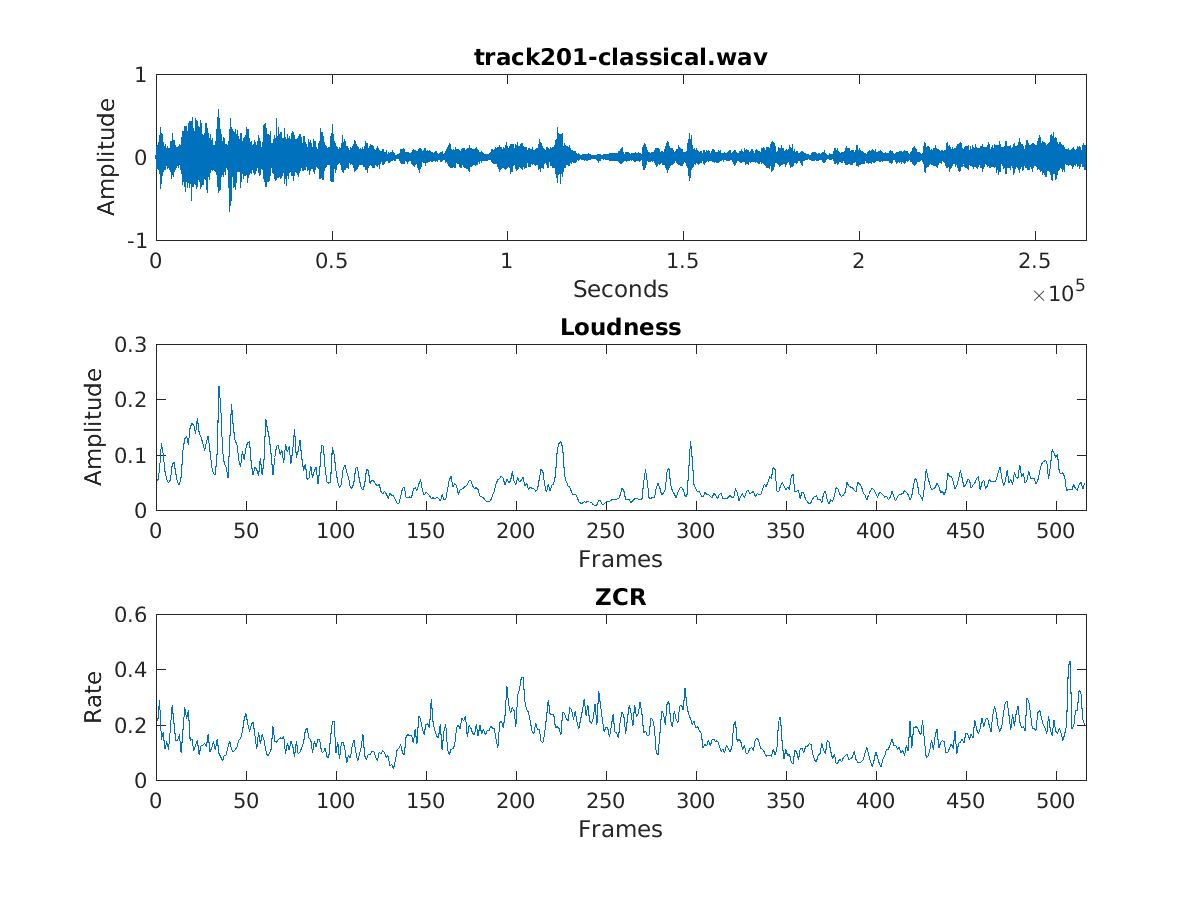
\includegraphics[width=.8\textwidth]{track201-classical-timedomain.png}
    \caption{track201-classical}
\end{figure}

The loudness graph simply takes a feature of the original soundtrack and essentially looks at the peak of the song at that moment in time. It is obvious what feature it holds, and in terms of determining genre, it does no better than using the original audio file. \\

For ZCR, since it is related to pitch height and noisiness, it is obvious that this is a much quieter song. This may be related to only a limited number of instruments, but is not a clear indication of genre. \\

\begin{figure}[H]
    \centering
    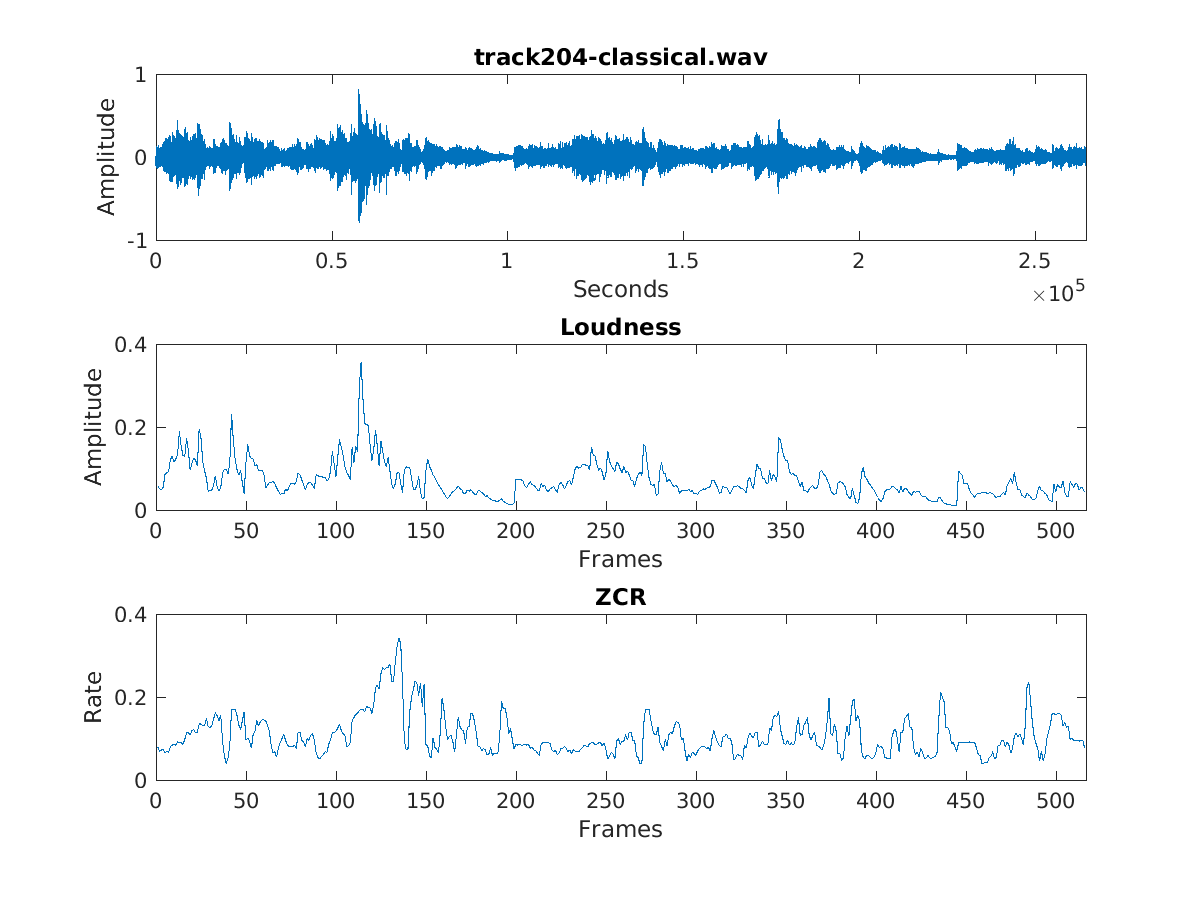
\includegraphics[width=.8\textwidth]{track204-classical-timedomain.png}
    \caption{track204-classical}
\end{figure}

Again, like the first classical track, the loudness graph demonstrates very similar, yet a bit more focused look at the amplitude of the song. \\

The ZCR follows the loudness very similarly in terms of amplitude. The large increase in sound at around the 100th frame is seen as an increase in the ZCR after 100 frames. There may or may not be a correlation between ZCR and the type of genre.

\begin{figure}[H]
    \centering
    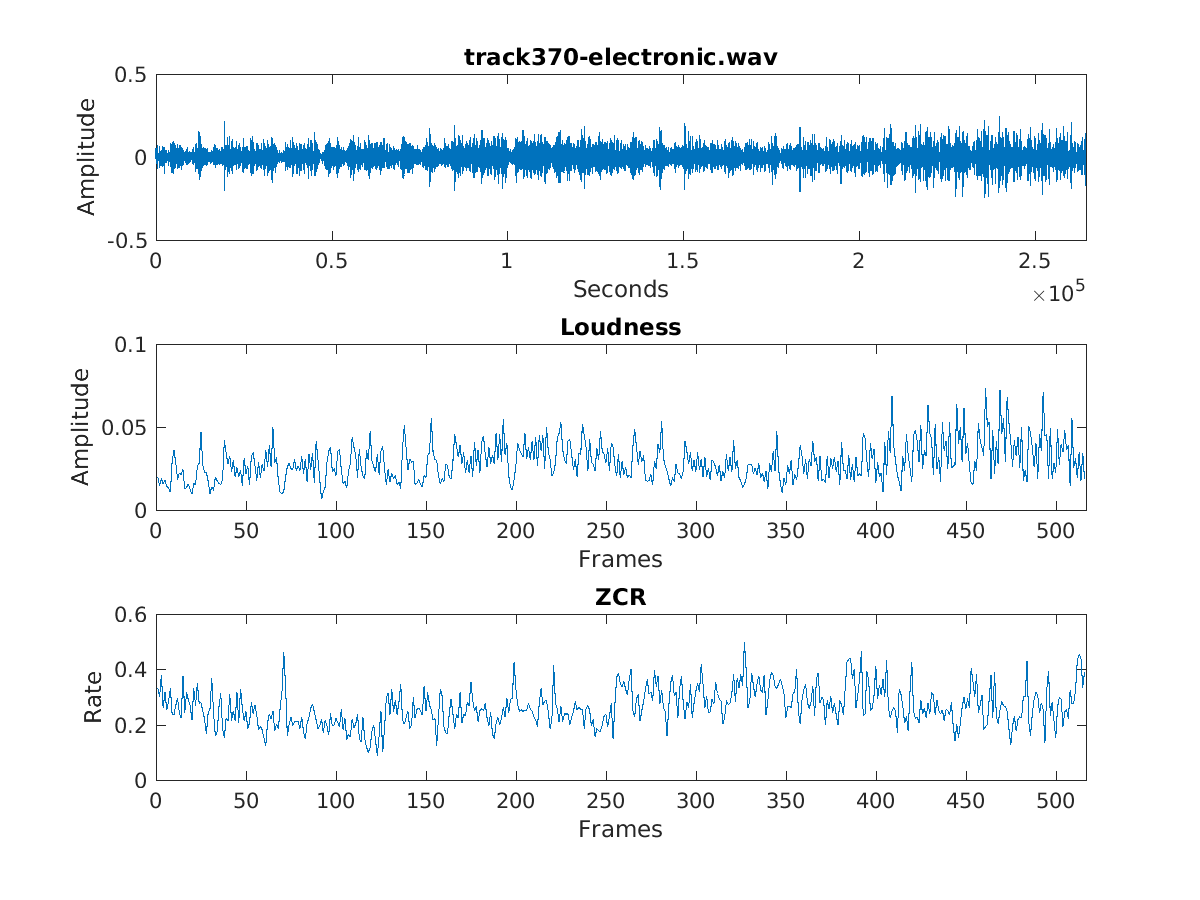
\includegraphics[width=.8\textwidth]{track370-electronic-timedomain.png}
    \caption{track370-electronic}
\end{figure}

There is nothing of interest to note in the loudness of the electronic track. There is not that much of a difference between it and the original audio.\\

An interesting note is the higher rates in the ZCR per frame. In electronic, there is a much larger number of zero-crossings. 

\begin{figure}[H]
    \centering
    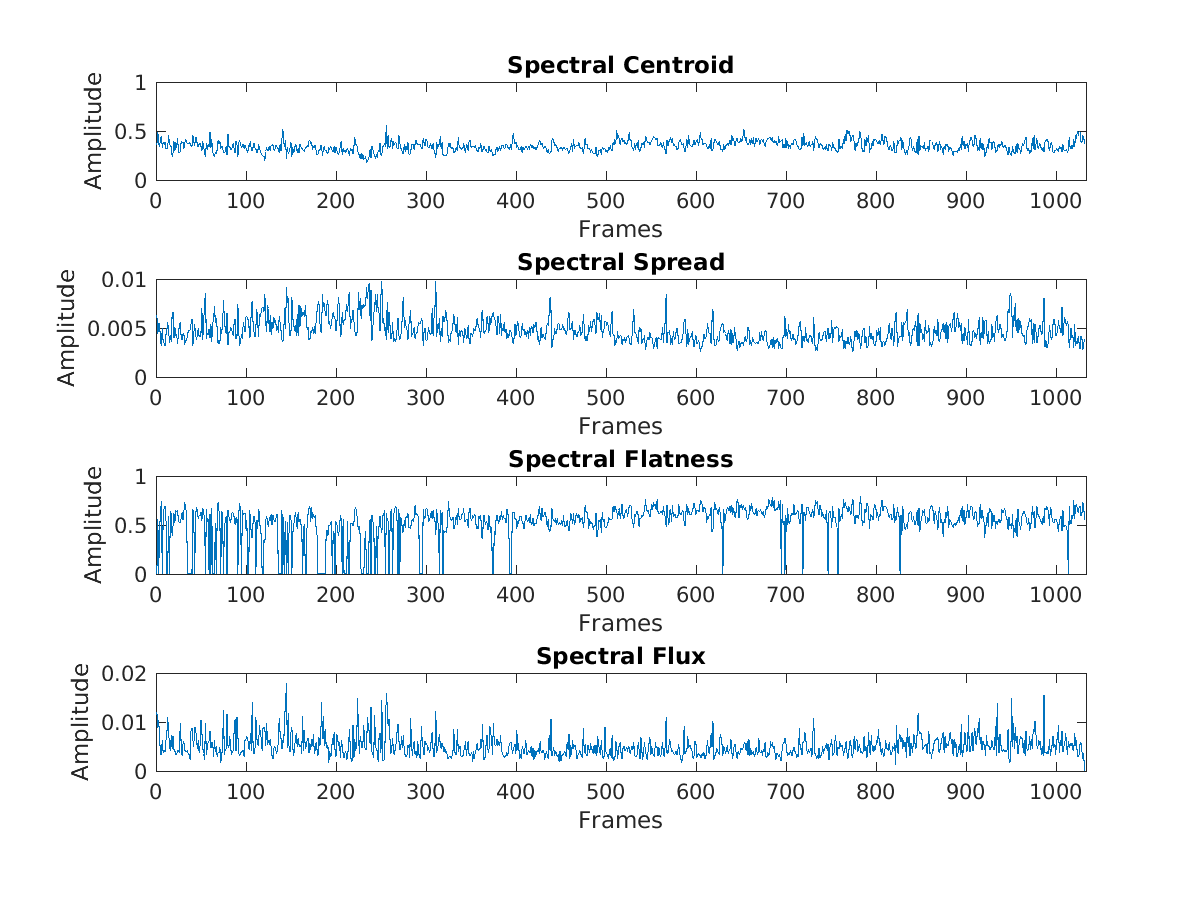
\includegraphics[width=.8\textwidth]{track396-electronic-timedomain.png}
    \caption{track396-electronic}
\end{figure}

The loudness illustrates the song has some sinusoidal component in the song and this follows suit to the ZCR. Unlike the other electronic track, there are no real similar patterns between these two songs of the same genre.


\begin{figure}[H]
    \centering
    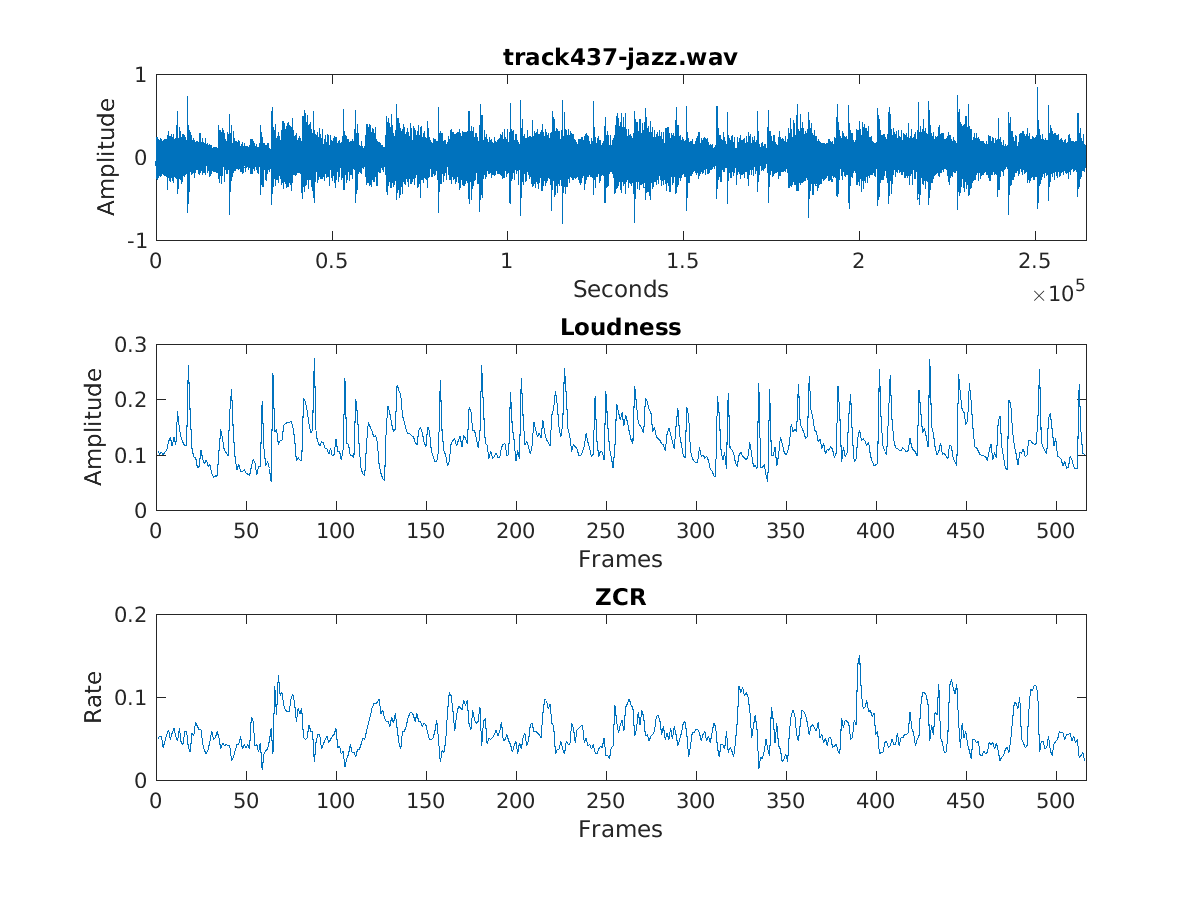
\includegraphics[width=.8\textwidth]{track437-jazz-timedomain.png}
    \caption{track437-jazz}
\end{figure}

Jazz may contain a special feature where are there momentary spikes in the amplitude of the song. The loudness graph demonstrates this feature, but the ZCR does not show any difference between itself and the classical tracks.

\begin{figure}[H]
    \centering
    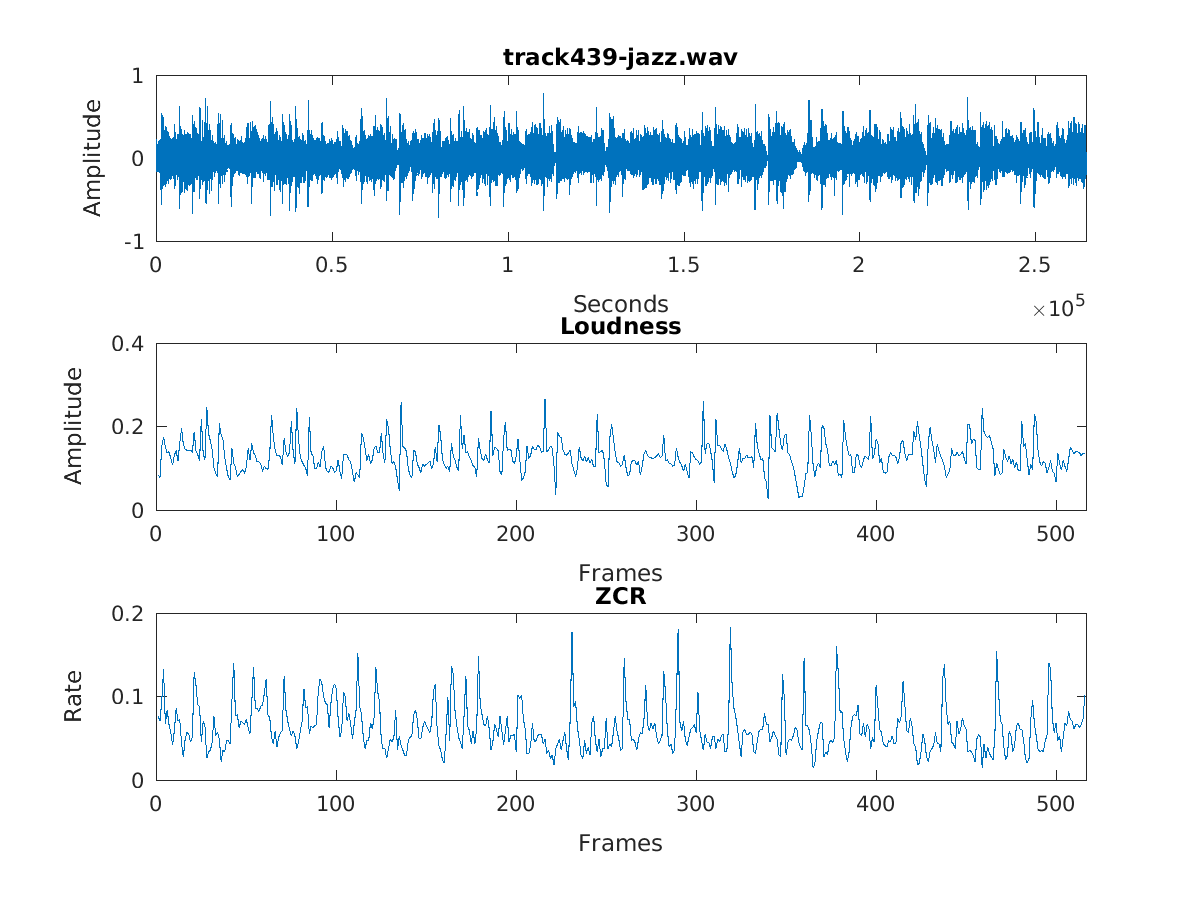
\includegraphics[width=.8\textwidth]{track439-jazz-timedomain.png}
    \caption{track437-jazz}
\end{figure}

Like the first jazz track, this track shares similar traits, where there are spikes that occur that produces loud noises. The ZCR for this track, however, also demonstrates some large changes in the rates during some of these moments. 


\begin{figure}[H]
    \centering
    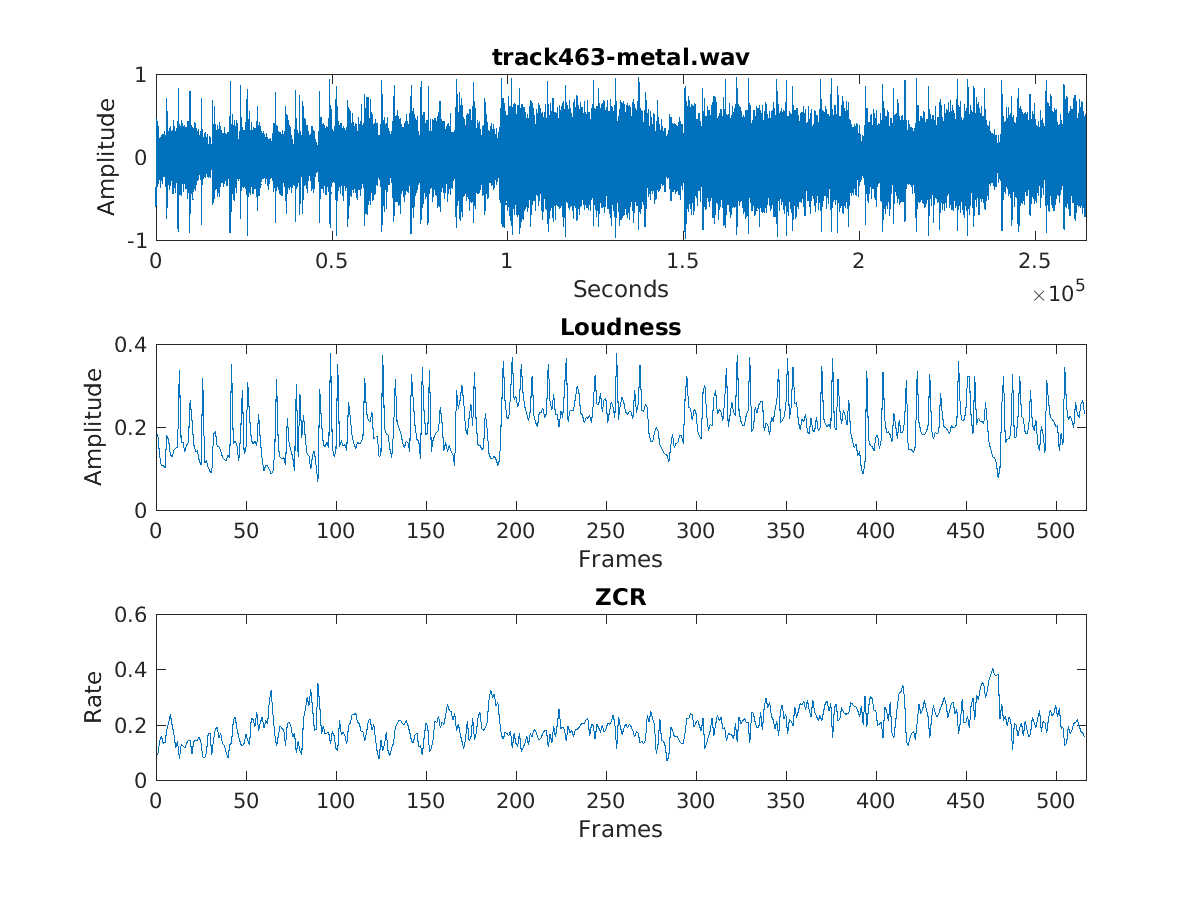
\includegraphics[width=.8\textwidth]{track463-metal-timedomain.png}
    \caption{track463-metal}
\end{figure}

Metal music is very loud, but does not seem to show very much change in the ZCR, similar to the classical tracks. 

\begin{figure}[H]
    \centering
    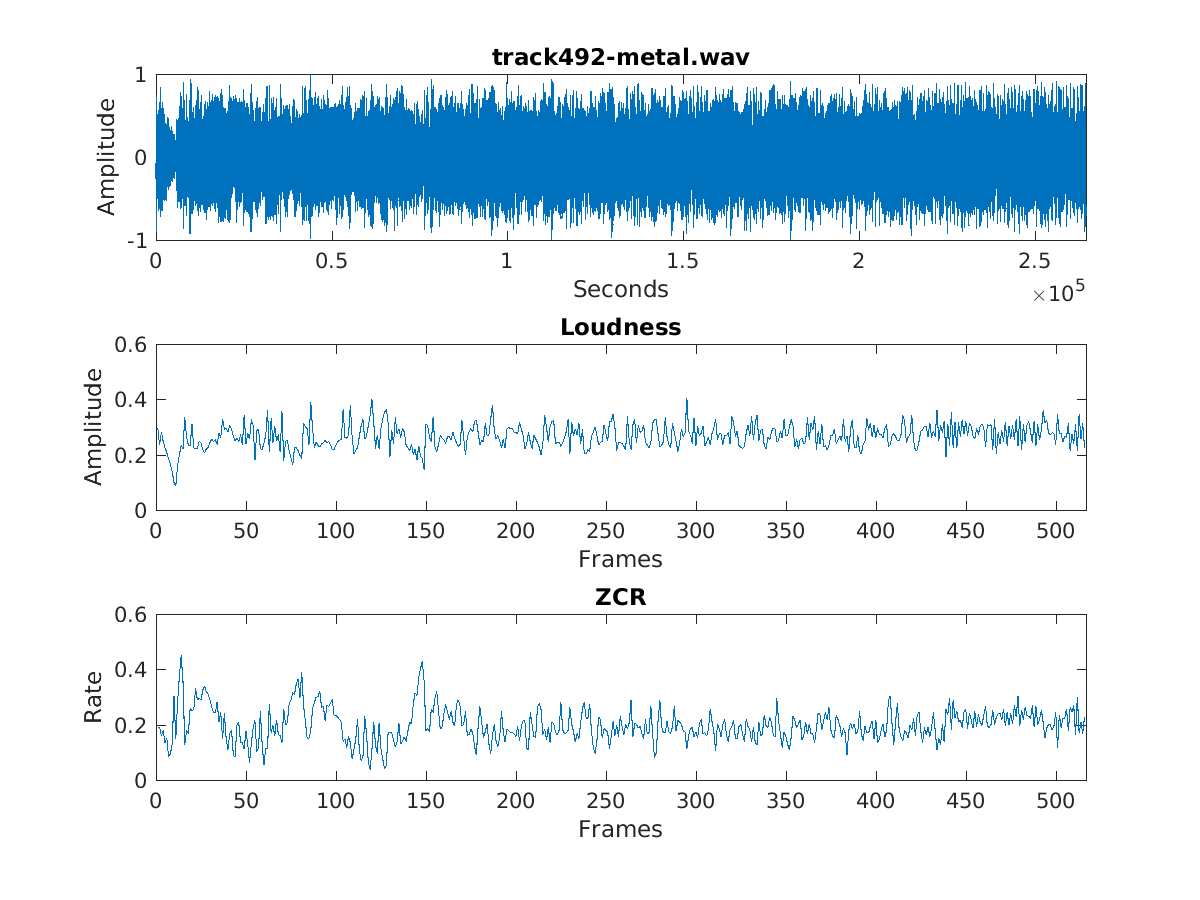
\includegraphics[width=.8\textwidth]{track492-metal-timedomain.png}
    \caption{track492-metal}
\end{figure}

Again, this metal track shares similarities to the previous track. 


\begin{figure}[H]
    \centering
    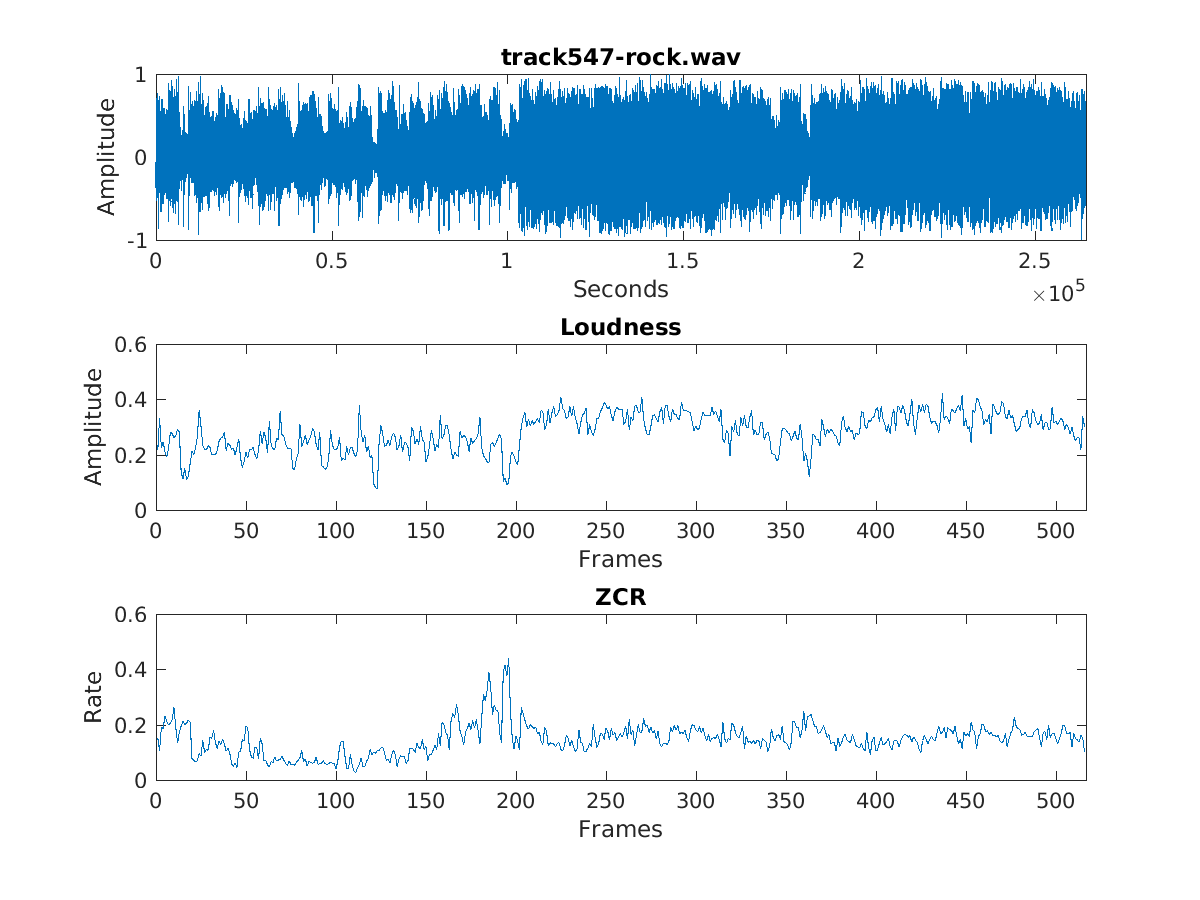
\includegraphics[width=.8\textwidth]{track547-rock-timedomain.png}
    \caption{track547-rock}
\end{figure}

The rock track shows some interesting features in all three graphs. There is a noticeable change in the song at around 200 frames where both the loudness and ZCR change. 

\begin{figure}[H]
    \centering
    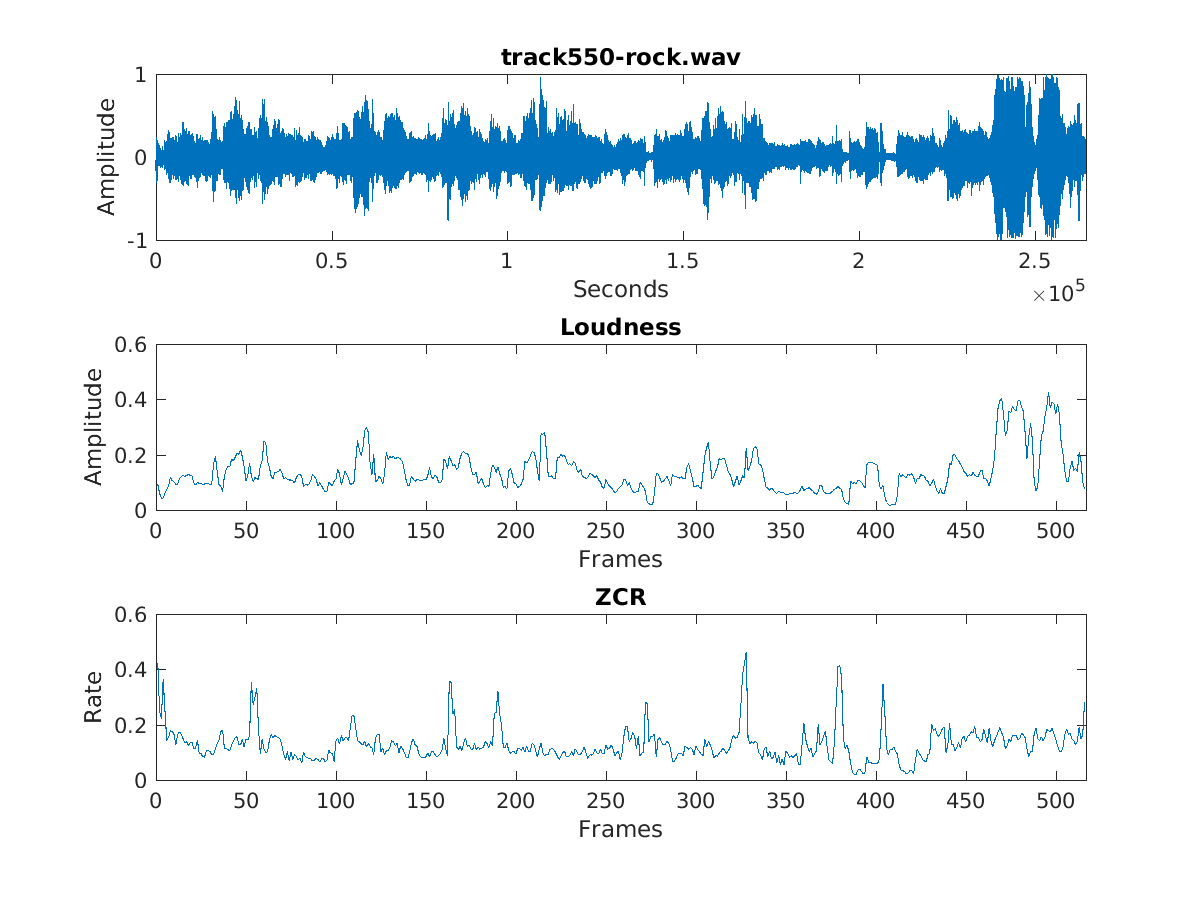
\includegraphics[width=.8\textwidth]{track550-rock-timedomain.png}
    \caption{track550-rock}
\end{figure}

This rock track is very different, but iterates the same facts: the loudness graph follows the audio signal, and the ZCR does not seem to have much correlation to the song. 


\begin{figure}[H]
    \centering
    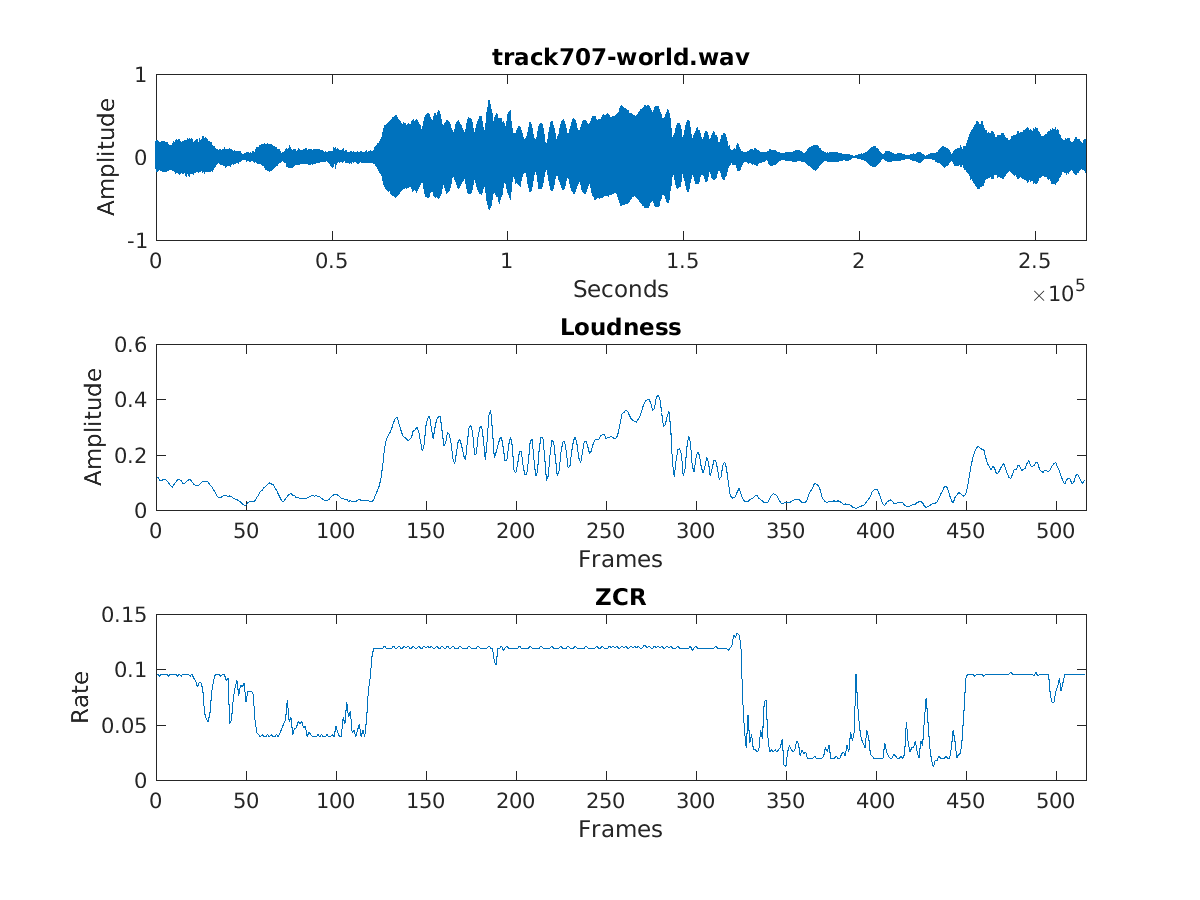
\includegraphics[width=.8\textwidth]{track707-world-timedomain.png}
    \caption{track707-world}
\end{figure}

The world track is very strange due to the constant noise it makes at the 125th frame. The loudness follows suit to the audio track, and the ZCR demonstrates that there is a consistent rate of zero-crossing, which may indicate this is of something like a sinusoidal. 


\begin{figure}[H]
    \centering
    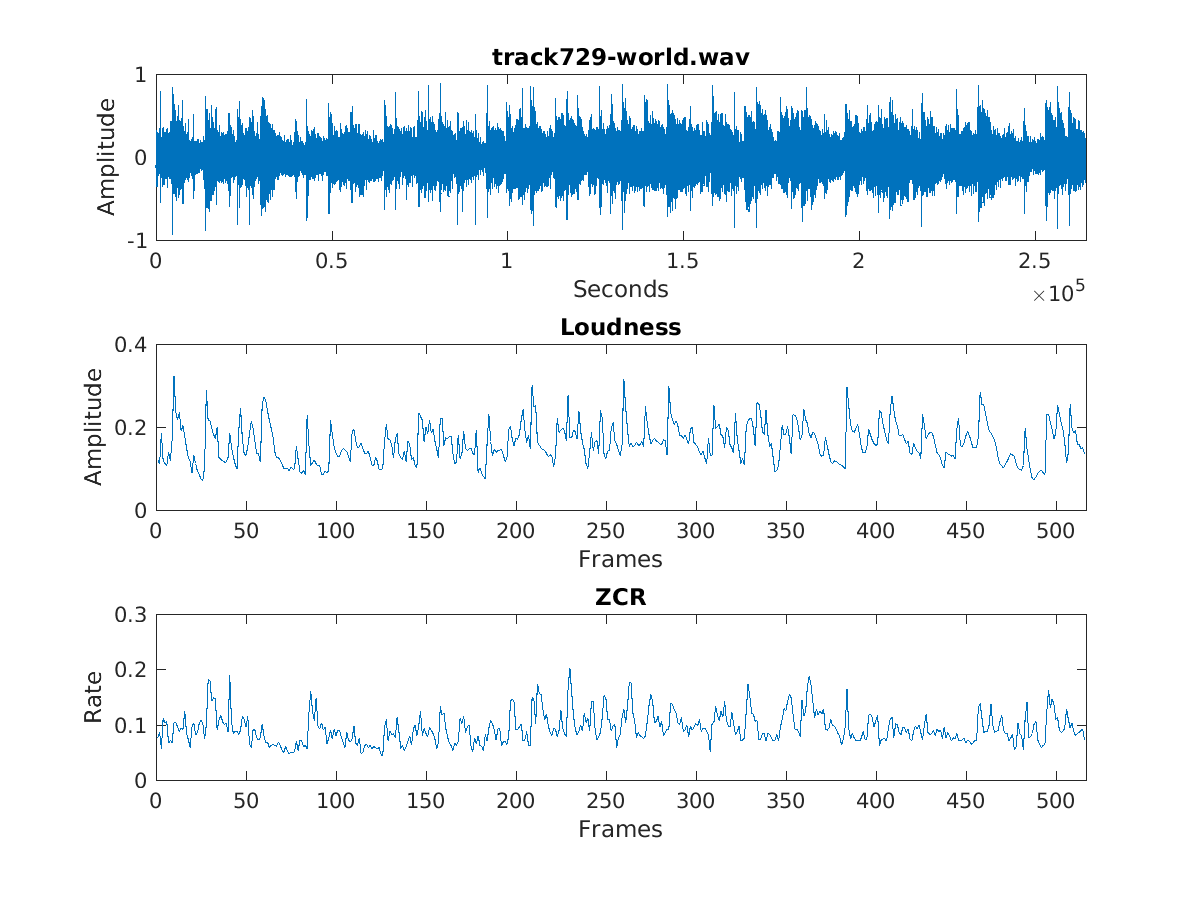
\includegraphics[width=.8\textwidth]{track729-world-timedomain.png}
    \caption{track729-world}
\end{figure}

The last world track shares a lot of similarities to the metal tracks, and it is not obvious where it is from. \\

\subsection{Conclusion: Loudness and ZCR}

Loudness and ZCR are both time domain analysis on the songs, but do not seem to provide enough detail on the songs to give direction to what type of genre it is. A classical song can be loud and abrupt like metal, and demonstrate similar loudness, but this is a poor indication of determining genres. \\

The ZCR also does not seem to give much input to genre as many of the ZCR could be mistaken for one genre to another. By only looking at the time domain, there is insufficient information given to do any analysis. \\


\section{FFT and Spectral Analysis}

\subsection{FFT}
The derivation of the Fourier transform of a cosine is as following:

\begin{equation}
x[n] = cos(w_0n), n \subset \mathbb{Z}
\end{equation}

\mth{
X(e^{jw}) &= \sum\limits_{n=-\infty}^{\infty} x[n]e^{-jwn}\\
&= \sum\limits_{n=-\infty}^{\infty} cos(w_0n)e^{-jwn}\\
&= \sum\limits_{n=-\infty}^{\infty} \frac{(e^{-jw_0n} + e^{jw_0n})}{2}e^{-jwn} \\
&= \sum\limits_{n=-\infty}^{\infty} \frac{(e^{-j(w_0-w)n} + e^{j(w_0-w)n})}{2} \\
&= \sum\limits_{n=-\infty}^{\infty} \frac{(e^{-j(w_0-w)n})}{2} + \sum\limits_{n=-\infty}^{\infty} \frac{(e^{j(w_0-w)n})}{2}
}

Because this is simply turning into the Fourier transform of two exponential functions, the Fourier transform simply turns into two deltas, centered at the fundamental frequency. \\

\begin{equation}
X(e^{jw}) = \sum\limits_{n=-\infty}^{\infty} (\delta(w-w_0) +\delta(w+w_0))\\
\end{equation}

For the derivation of the Fourier transform the following:

\begin{equation}
y[n] = x[n]w[n-\frac{N}{2}
\end{equation}

You can use the convolution property to get the Fourier transform:

\begin{equation}
Y(e^{jw}) = X(e^{jw})*W(e^{jw})e^{-jw\frac{N}{2}}
\end{equation}

Since w contains a time shift this results in an extra exponential component. \\




\subsection{Windowing}

The windowing script generates a 100 Hz sine wave that is windowed with the three type of windowing filters.

\subsubsection{Windowing Code}
\lstinputlisting[language=Matlab]{../windowing.m} 

\begin{figure}[H]
    \centering
    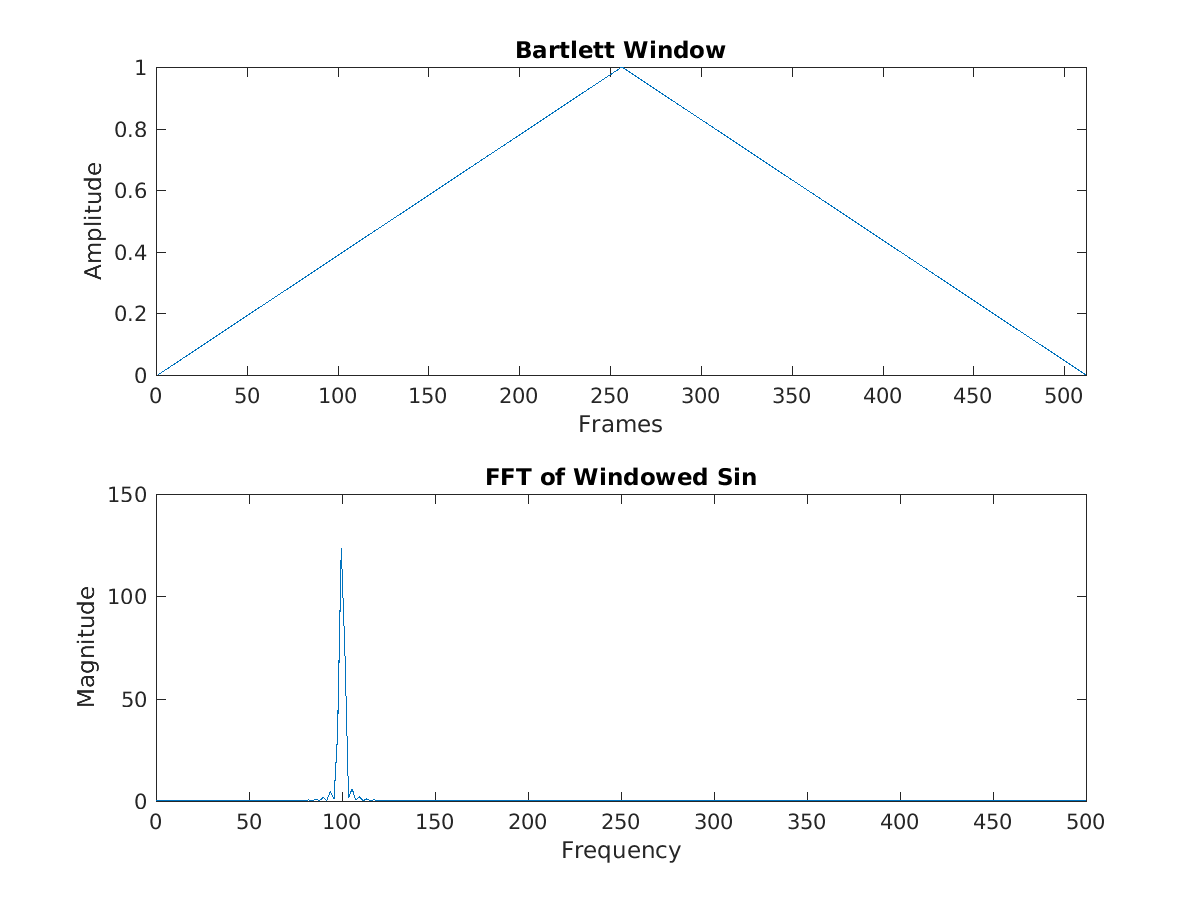
\includegraphics[width=.8\textwidth]{bartlett-sin.png}
    \caption{Bartlett}
\end{figure}

The Bartlett window has some small oscillations that occur right before and after 100 Hz. This makes Bartlett a little less desirable since the filtered signal is not as smooth.

\begin{figure}[H]
    \centering
    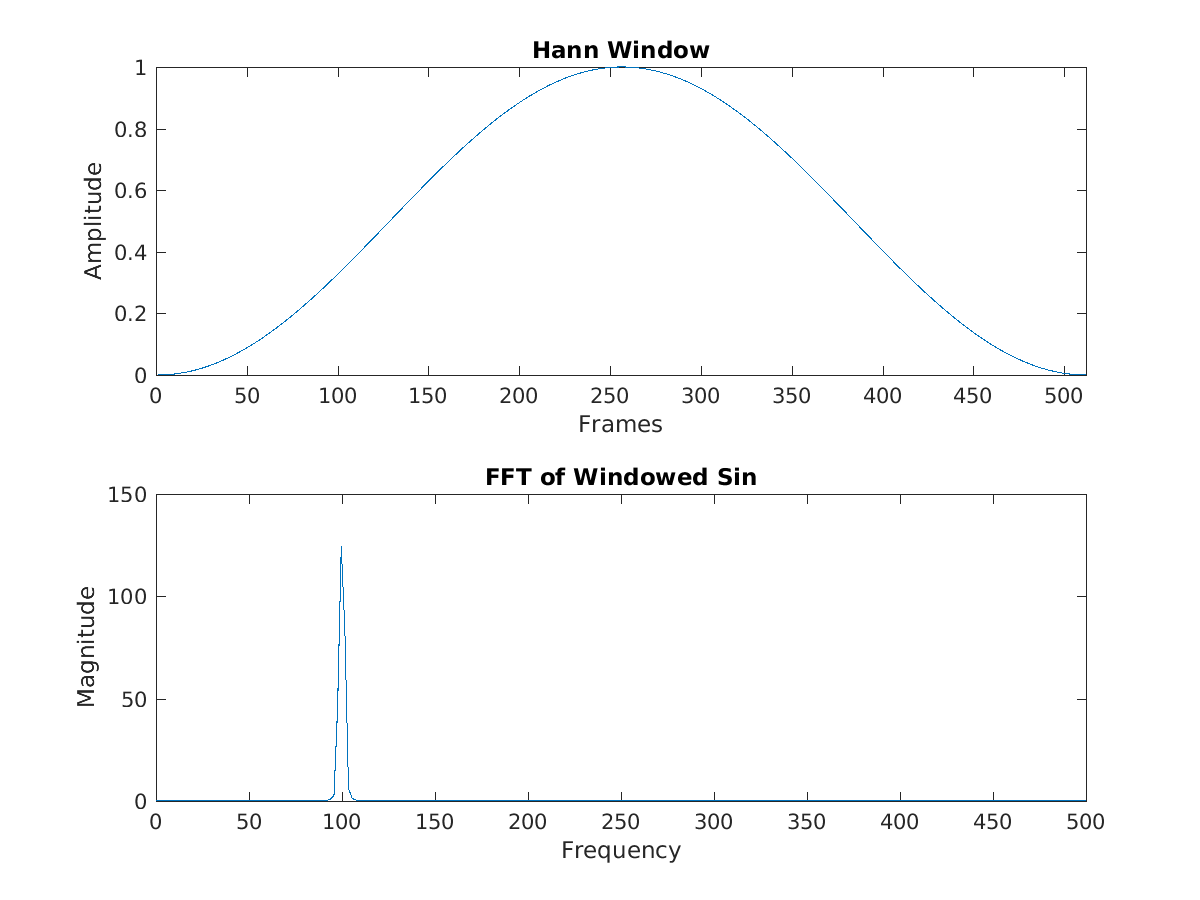
\includegraphics[width=.8\textwidth]{hann-sin.png}
    \caption{Hann}
\end{figure}

The Hann window does a much better job than the Bartlett window, but the Kaiser does a better job with really getting the 100 Hz. 

\begin{figure}[H]
    \centering
    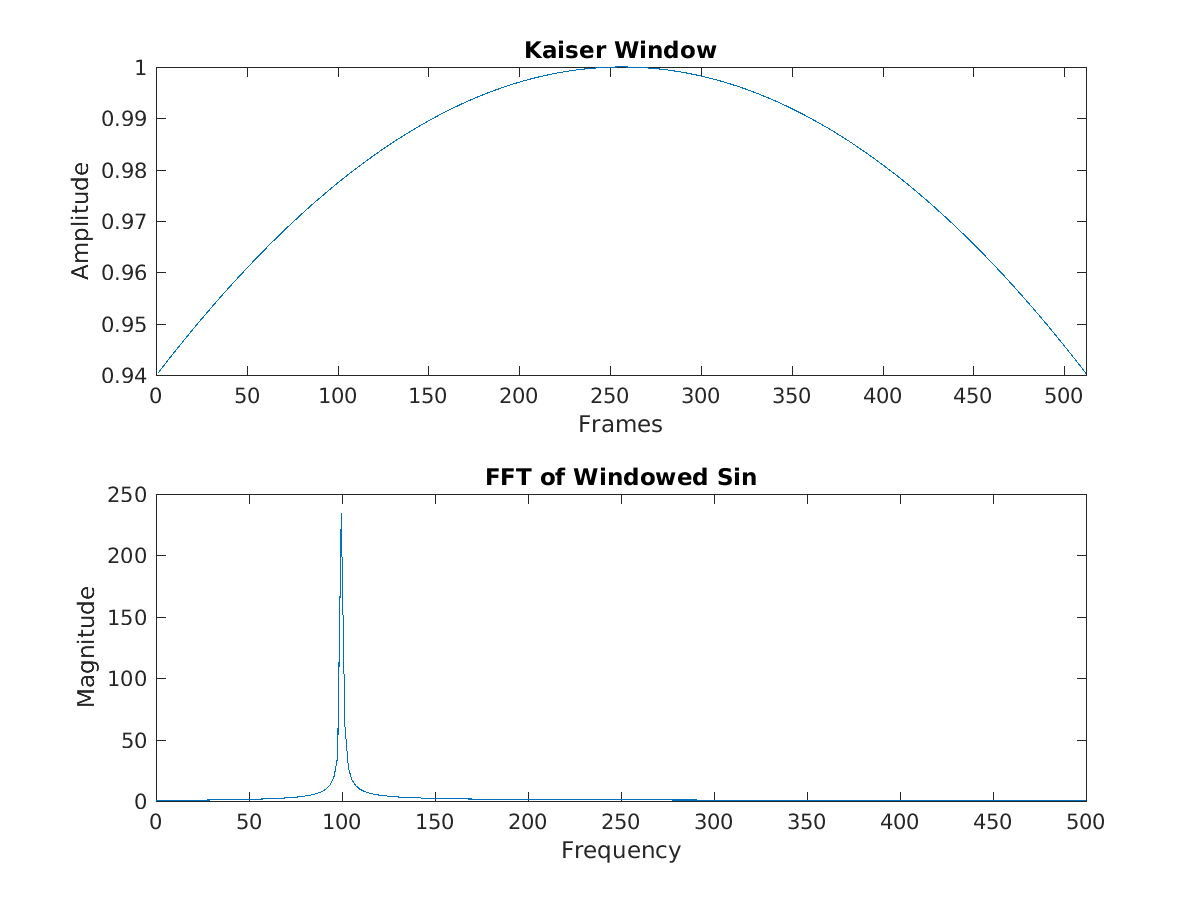
\includegraphics[width=.8\textwidth]{kaiser-sin.png}
    \caption{Kaiser}
\end{figure}

Compared to the Hann window, the Kaiser window slopes a little bit near 100 Hz, but when looking at 100 Hz, the width of the peak is considerably smaller than Bartlett and Hann. 


\subsection{Spectral Analysis Code}

The spectrogram was generated using the following Matlab code.
\lstinputlisting[language=Matlab]{../plotspectrogram.m}

The spectral analysis of the centroid, spread, flatness, and flux were found using the following Matlab code. 
\lstinputlisting[language=Matlab]{../spectralAnalysis.m}

\pagebreak

\begin{figure}[H]
    \centering
    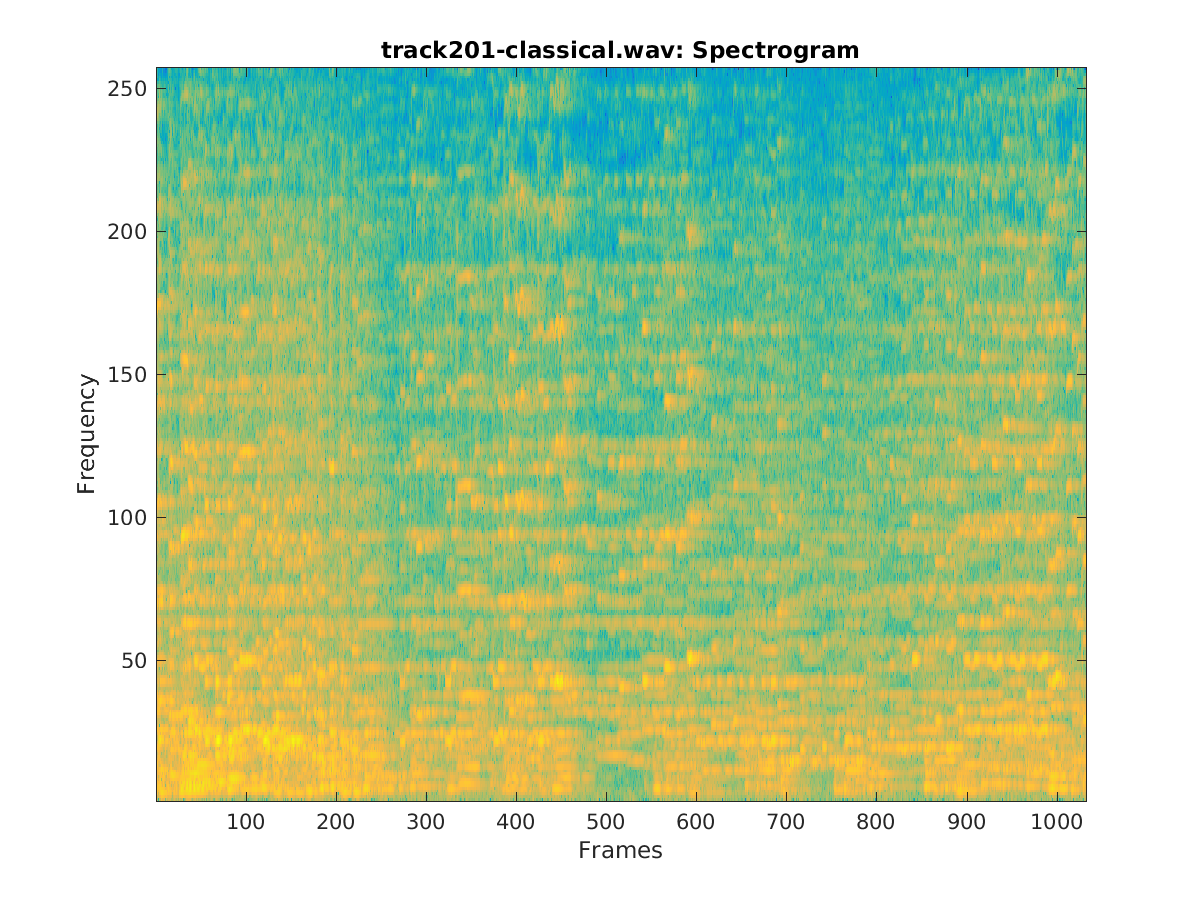
\includegraphics[width=.75\textwidth]{track201-classical-specto.png}
    \caption{track201-classical}
\end{figure}


\begin{figure}[H]
    \centering
    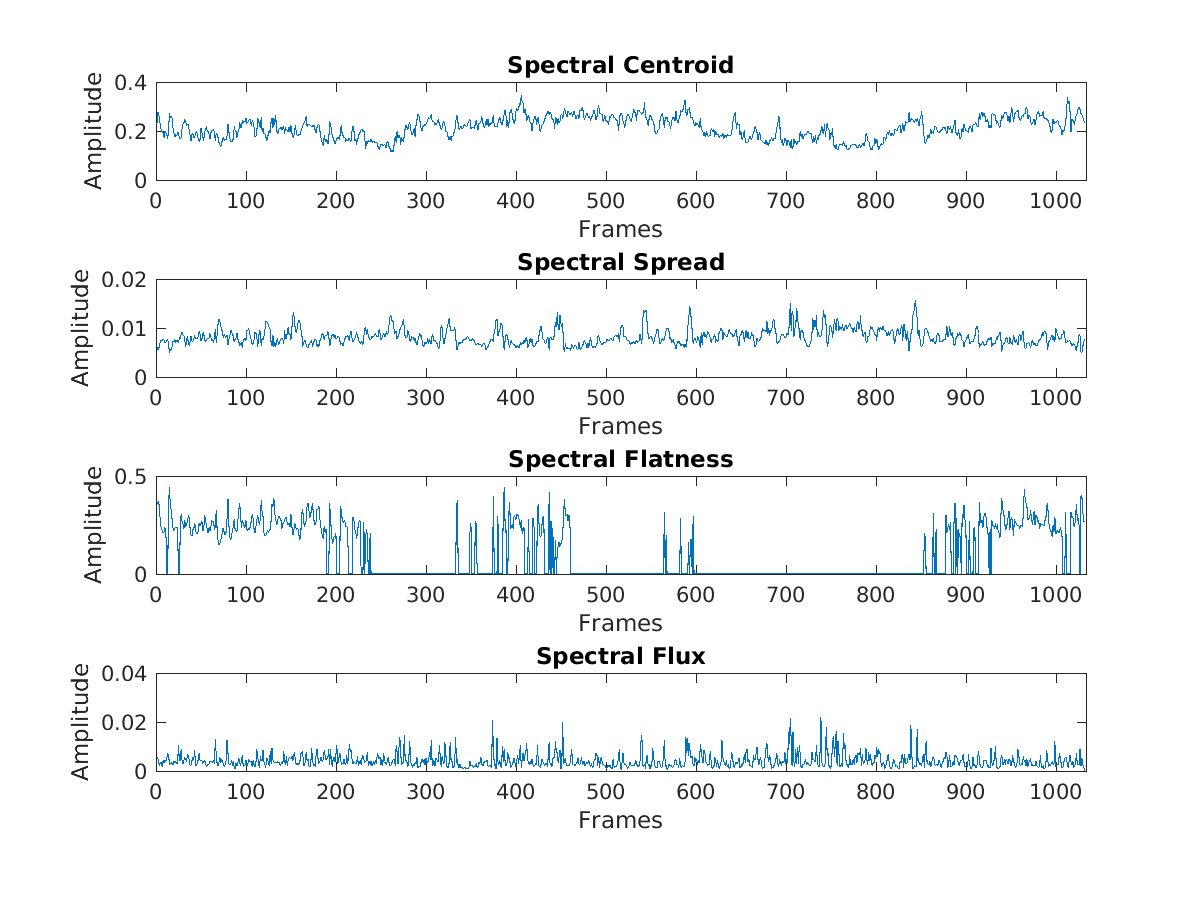
\includegraphics[width=\textwidth]{track201-classical-spectral.png}
    \caption{track201-classical}
\end{figure}

Its very difficult to be able to tell at which part of the song the spectrogram is displaying. The range of frequencies make sense for the type of genre being played, but it is hard to tell what is being played exactly. \\

The centroid demonstrates the rising and falling of the center tune of the song. The spread shows the spread of other frequencies in the song. The spread is close to 0 and thus means that that the spread of frequencies are mostly small. The classical track is less noisier than the other genres. \\

The flatness graph shows moments of the song where the frames are significantly quieter than the rest, such as frames 250 and 500. These moments are parts that sound tonal. \\

For flux, the low values means that there are not that many changes in the spectrogram from frame to frame. Classical songs may not have that dramatic changes and it can be expected to see such a low flux. 


\pagebreak

\begin{figure}[H]
    \centering
    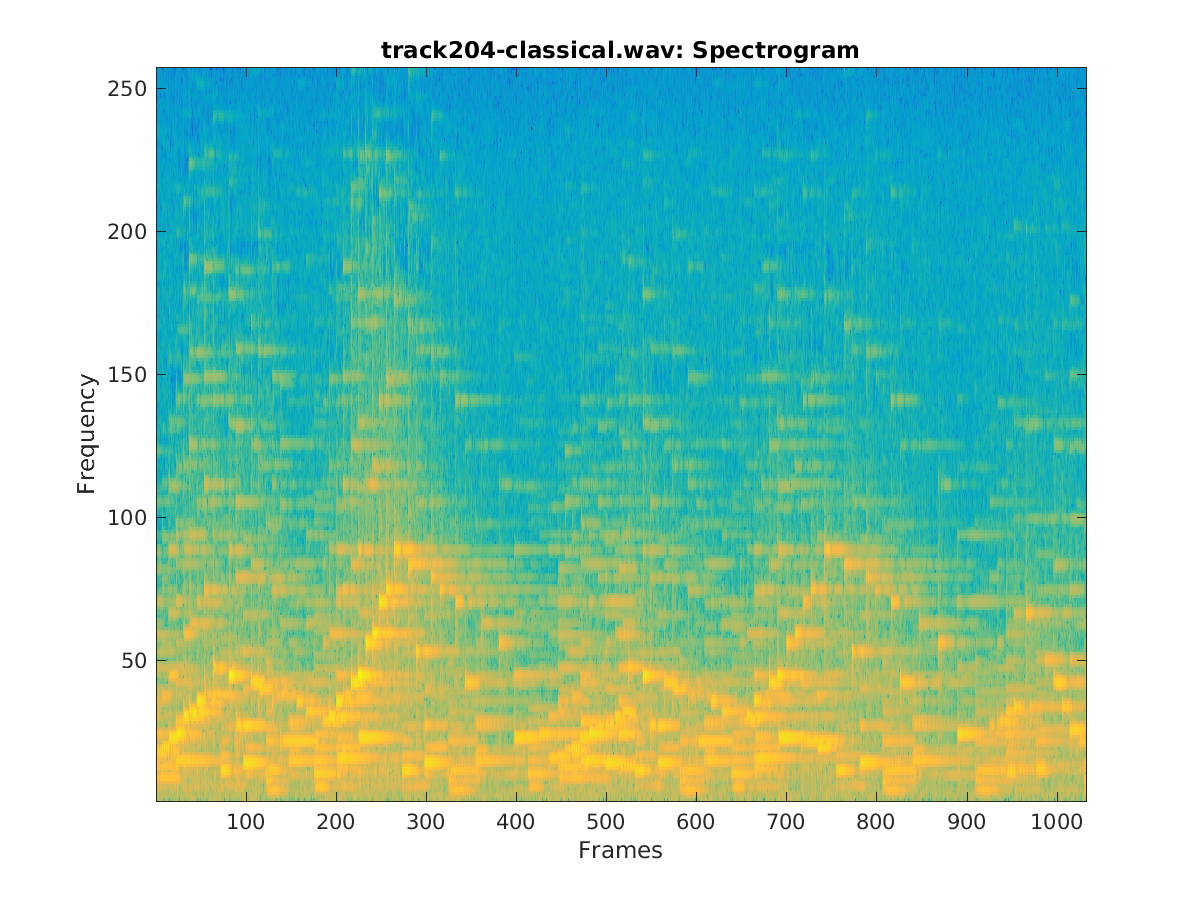
\includegraphics[width=.75\textwidth]{track204-classical-specto.png}
    \caption{track204-classical}
\end{figure}

\begin{figure}[H]
    \centering
    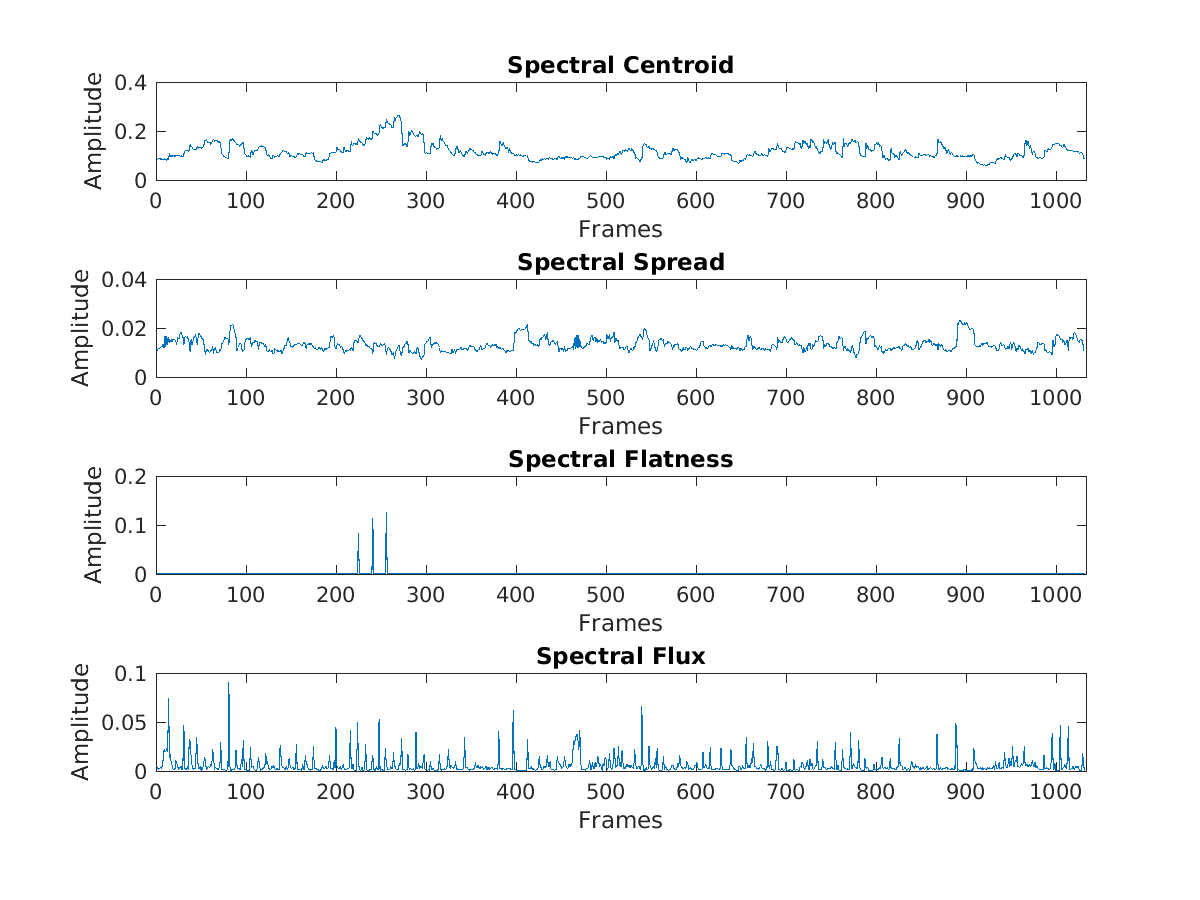
\includegraphics[width=\textwidth]{track204-classical-spectral.png}
    \caption{track204-classical}
\end{figure}

\pagebreak

This piano piece is easily seen in the spectrogram. Each note being played can be seen and it is, for the most part, easy to keep track of what is occurring through the song. \\

The centroid is very unique as it actually follows the piano notes that are being played. The spread is also mostly flat since there is not that many addition frequencies being played in the same time. This demonstrates that for genres that play specific tunes, these two are a good way of possibly detecting genres. \\

The flatness also shows this fact because since piano music is not very noisy and only contains the harmonics of the notes you play, there is a very low expected flatness. \\

The flux is dramatic because the notes that are being played frame to frame are different and thus, the flux shows this sudden change of each note. 

\pagebreak

\begin{figure}[H]
    \centering
    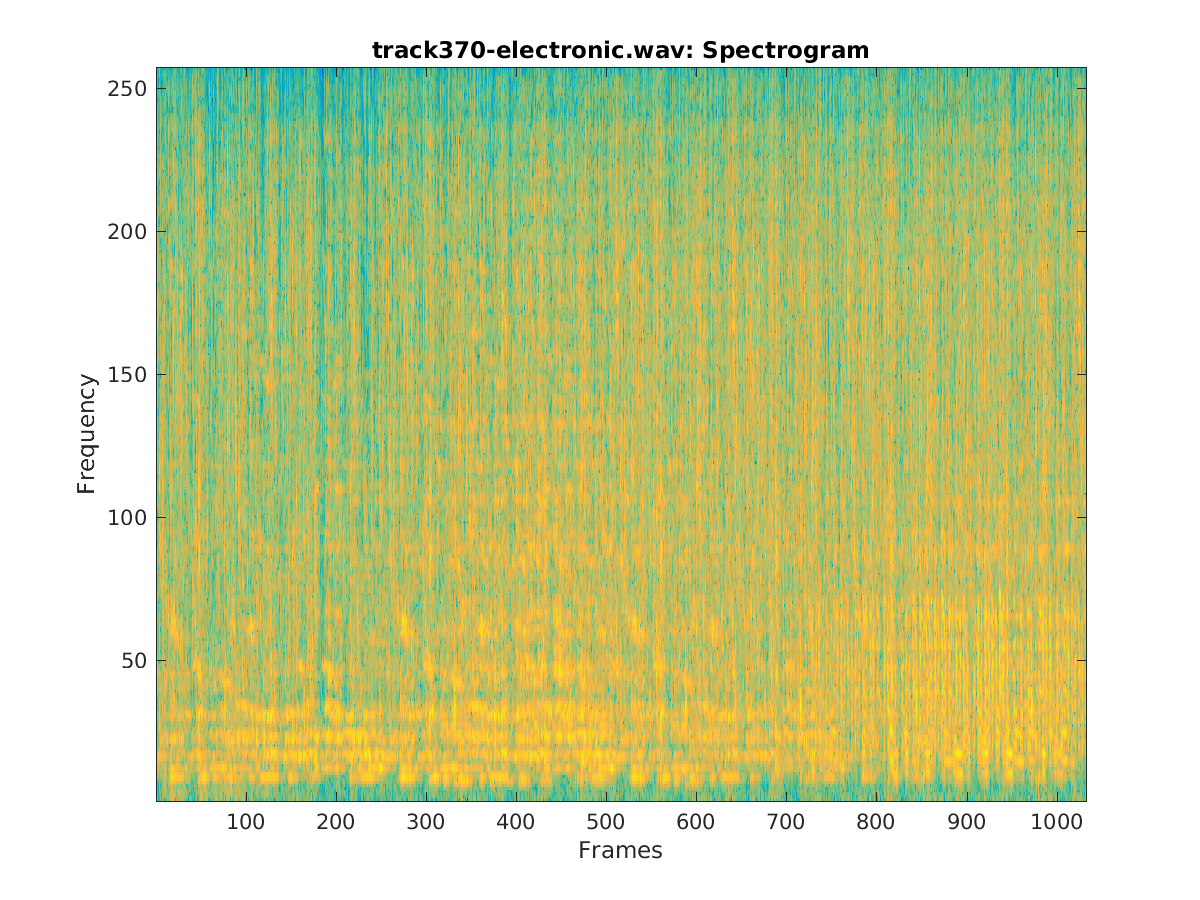
\includegraphics[width=.75\textwidth]{track370-electronic-specto.png}
    \caption{track370-electronic}
\end{figure}

\begin{figure}[H]
    \centering
    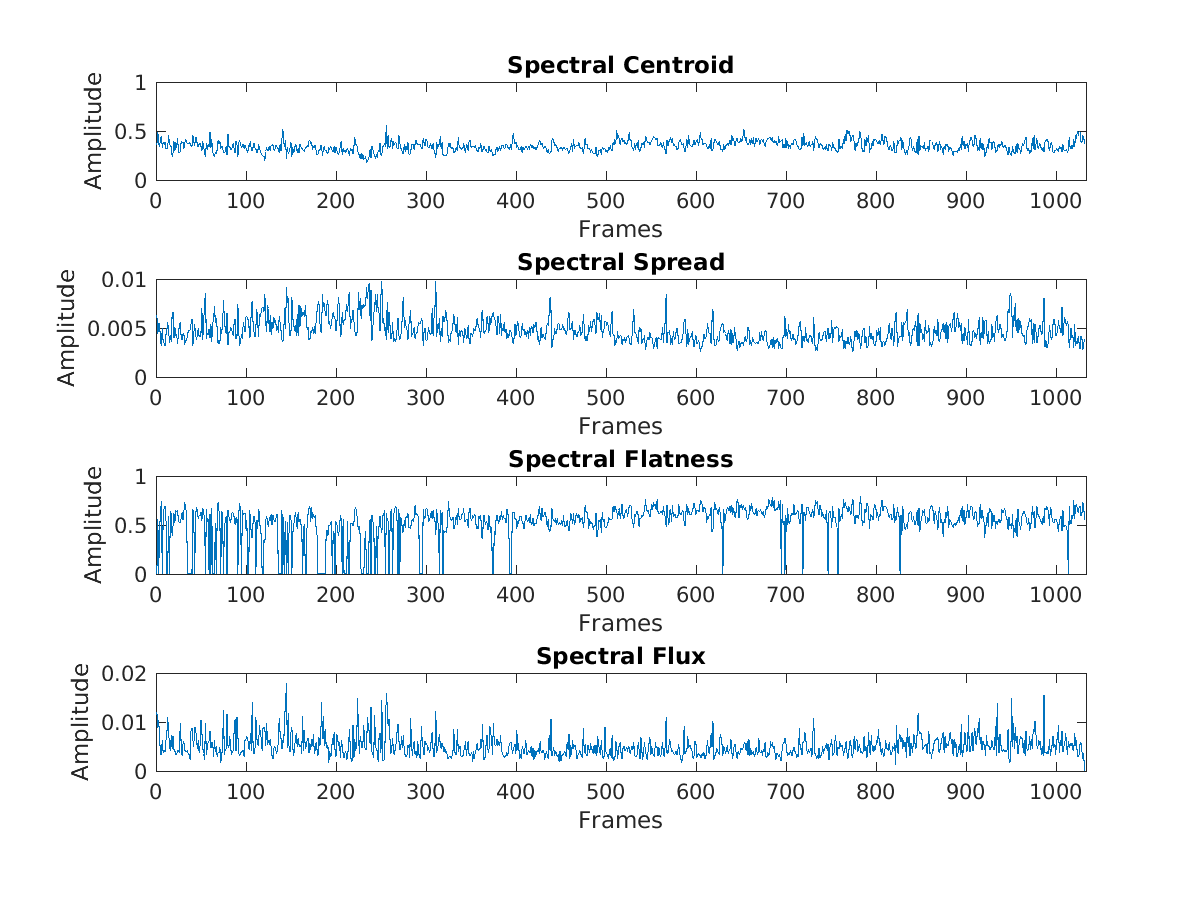
\includegraphics[width=1\textwidth]{track370-electronic-spectral.png}
    \caption{track370-electronic}
\end{figure}

There is not much to say about the spectrogram because the entire clip is just a bunch of noise. The spectrogram is very noisy and there is just a huge spread of frequencies throughout all the frames. \\

The centroid is in the center and it seems right to be so because of how much noise there is in the audio track. There really isn't one place of power in the frequency spectrum. As seen in the spread, this follows because there is a wide number of frequencies being played at the same time. \\

The spectral flatness is not very flat at all. Again, this makes sense considering how noisy the signal is. \\

The flux of this track is constantly changing, most likely due to the massive amount of noise the signal contains. \\

\pagebreak

\begin{figure}[H]
    \centering
    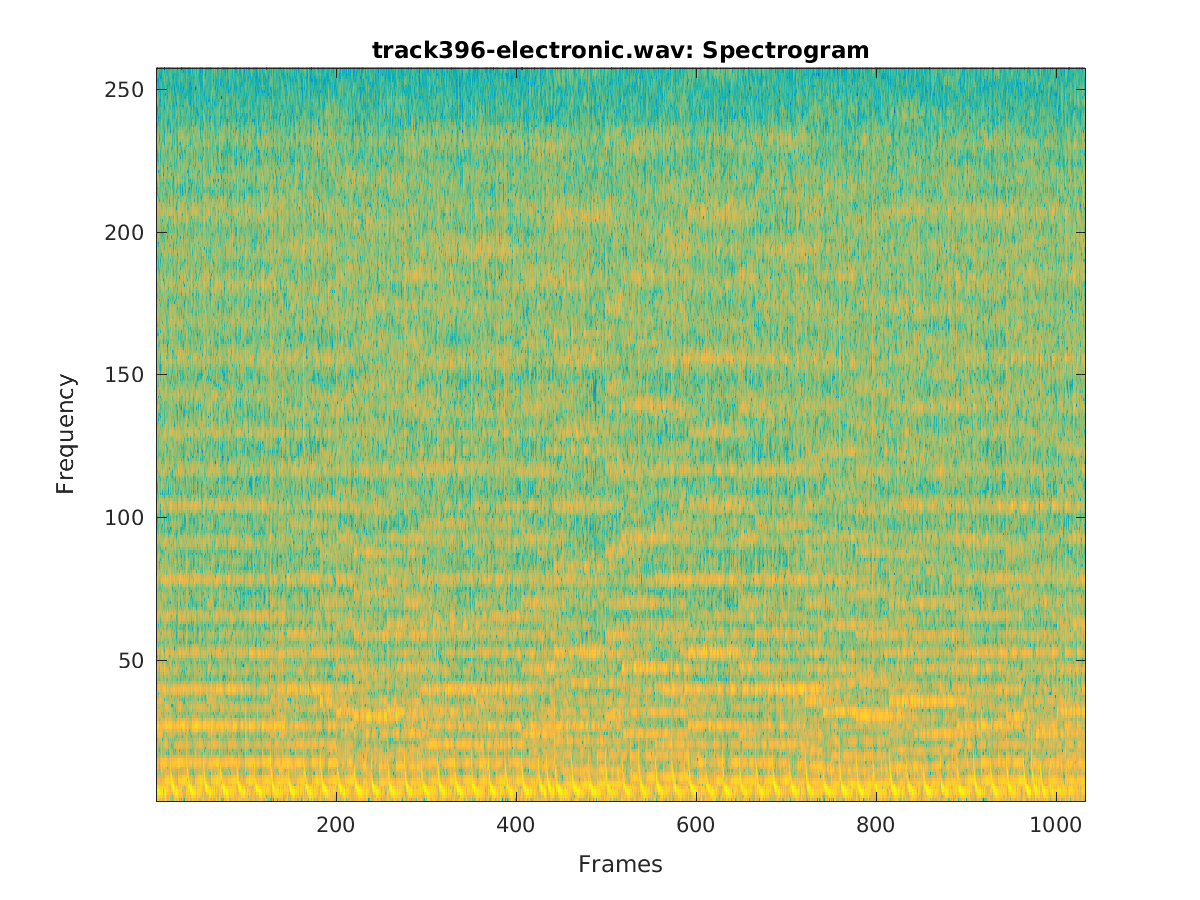
\includegraphics[width=.75\textwidth]{track396-electronic-specto.png}
    \caption{track396-electronic}
\end{figure}


\begin{figure}[H]
    \centering
    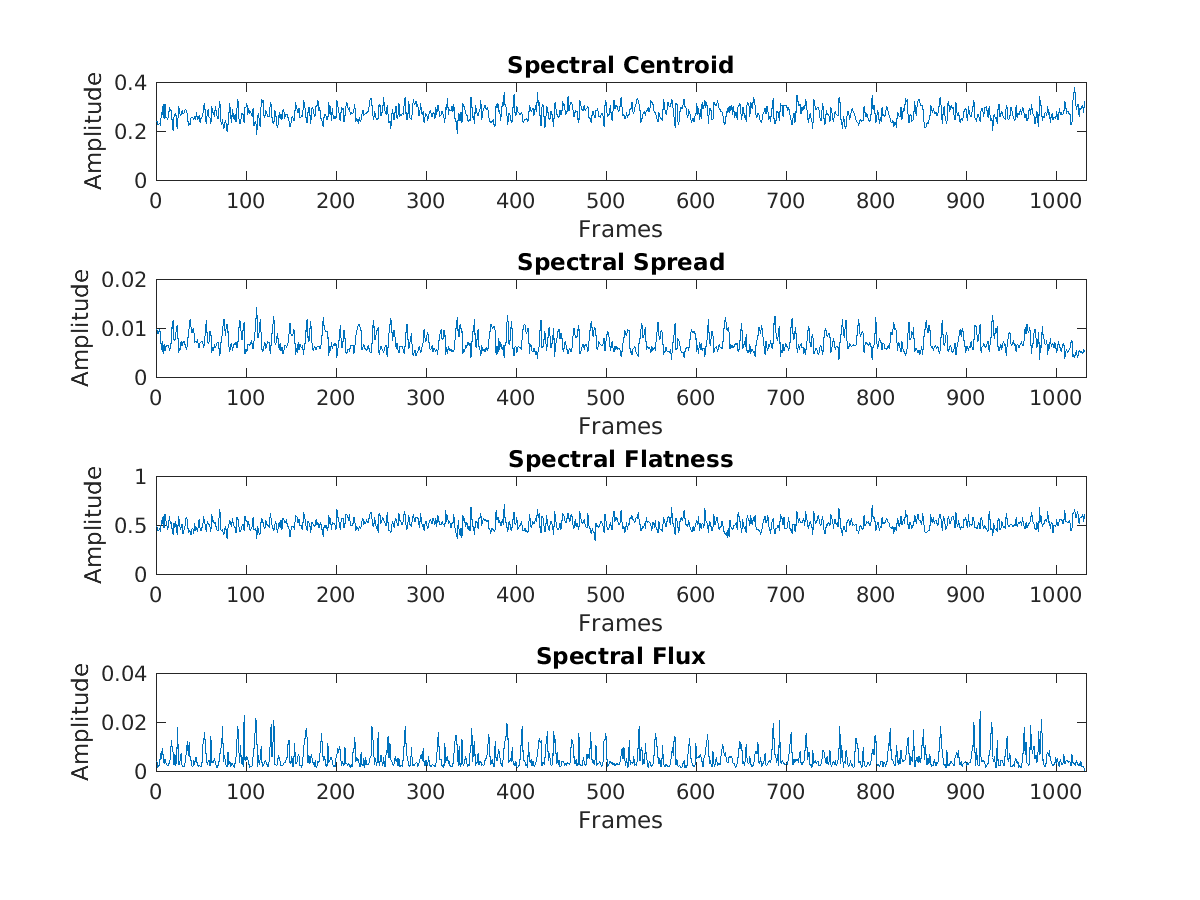
\includegraphics[width=\textwidth]{track396-electronic-spectral.png}
    \caption{track396-electronic}
\end{figure}

\pagebreak

This electronic track has a lot more consistencies than the previous track. The spectrogram makes a lot of sense and it can be heard what is happening. The beat of the song is seen consistently and can be tracked through the spectrogram. \\

Both the centroid and the spread are consistent, hovering around the same values over all the frames. This may point out a pattern that is happening with most electronic music that has a consistent beat playing. This gives the opportunity to realize that centroid and spread may have indications to what type of music is being played. \\

Flatness is mostly noisy, as seen in the spectrogram. There are several frequencies being played, but in comparison to other tracks, is not necessarily as bad. \\

For flux, it follows the pattern with centroid, spread, and flatness with consistent patterns on the frames. 

\pagebreak

\begin{figure}[H]
    \centering
    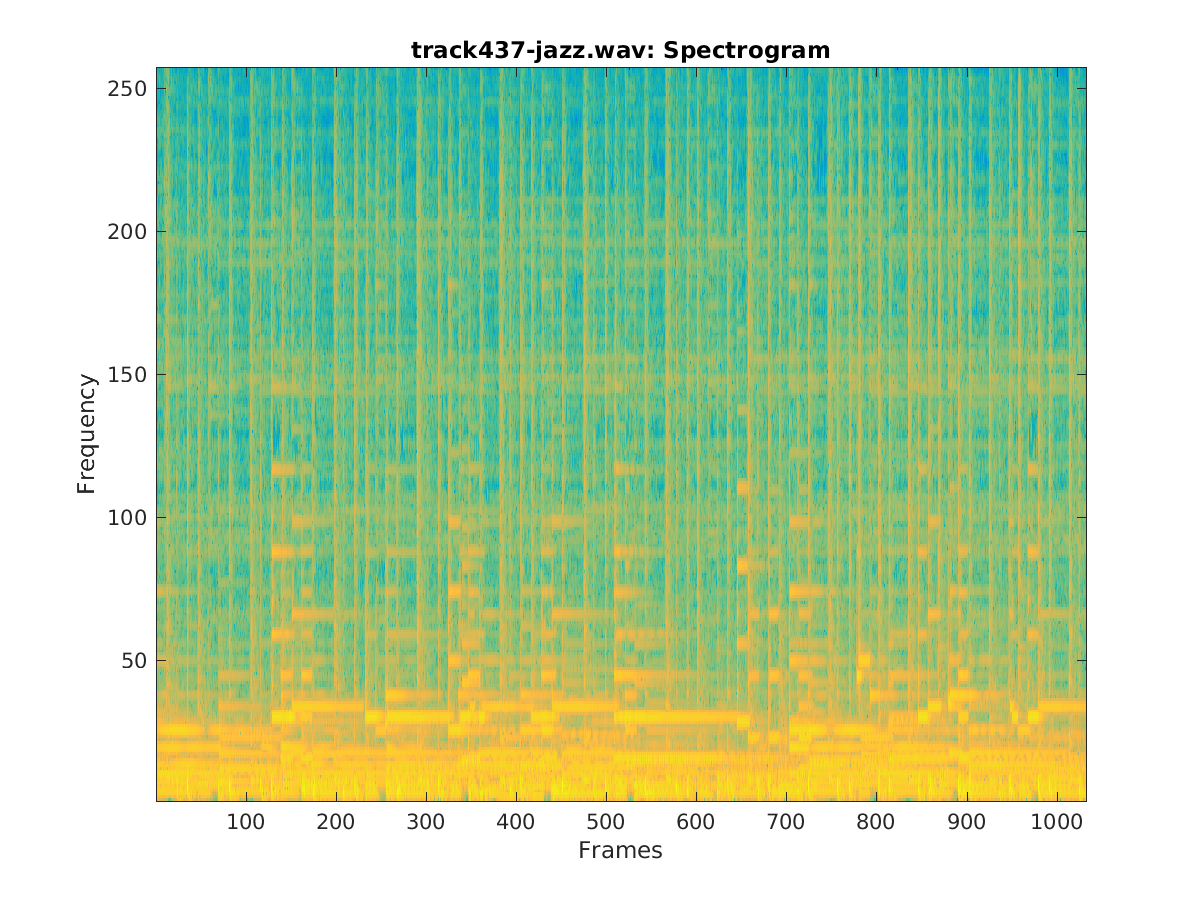
\includegraphics[width=.75\textwidth]{track437-jazz-specto.png}
    \caption{track437-jazz}
\end{figure}

\begin{figure}[H]
    \centering
    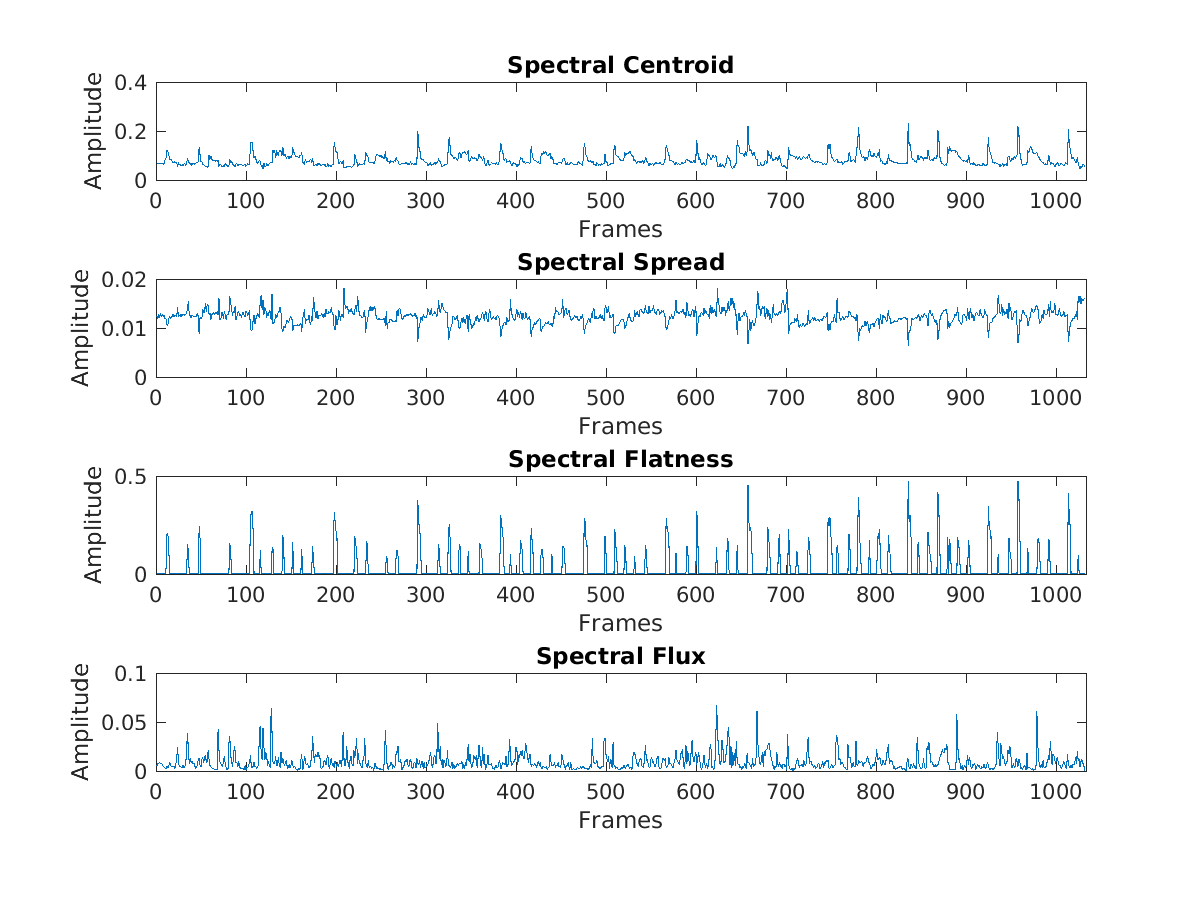
\includegraphics[width=\textwidth]{track437-jazz-spectral.png}
    \caption{track437-jazz}
\end{figure}

\pagebreak

A feature between all the tracks is the lower frequencies are all of higher magnitude. This is a possible weakness of using the spectrogram because it is not filtered and unwanted signals may be going through, causing a majority of the desired information to disappear. \\

The spectral centroid shows spikes in the sudden increase in power in the other bands at the specific frames. The spread also follows suits. So far, in general, the more consistent the centroid is, the purer the tone is. The spread represents that there is a broader power of frequencies being played at the same time. \\

Unlike the other tracks, there is a high increase in the flatness throughout the song. The instruments may be causing the audio to be very noisy when played. \\

The changes in the frequency spectrum follows through the flux as well. 

\pagebreak

\begin{figure}[H]
    \centering
    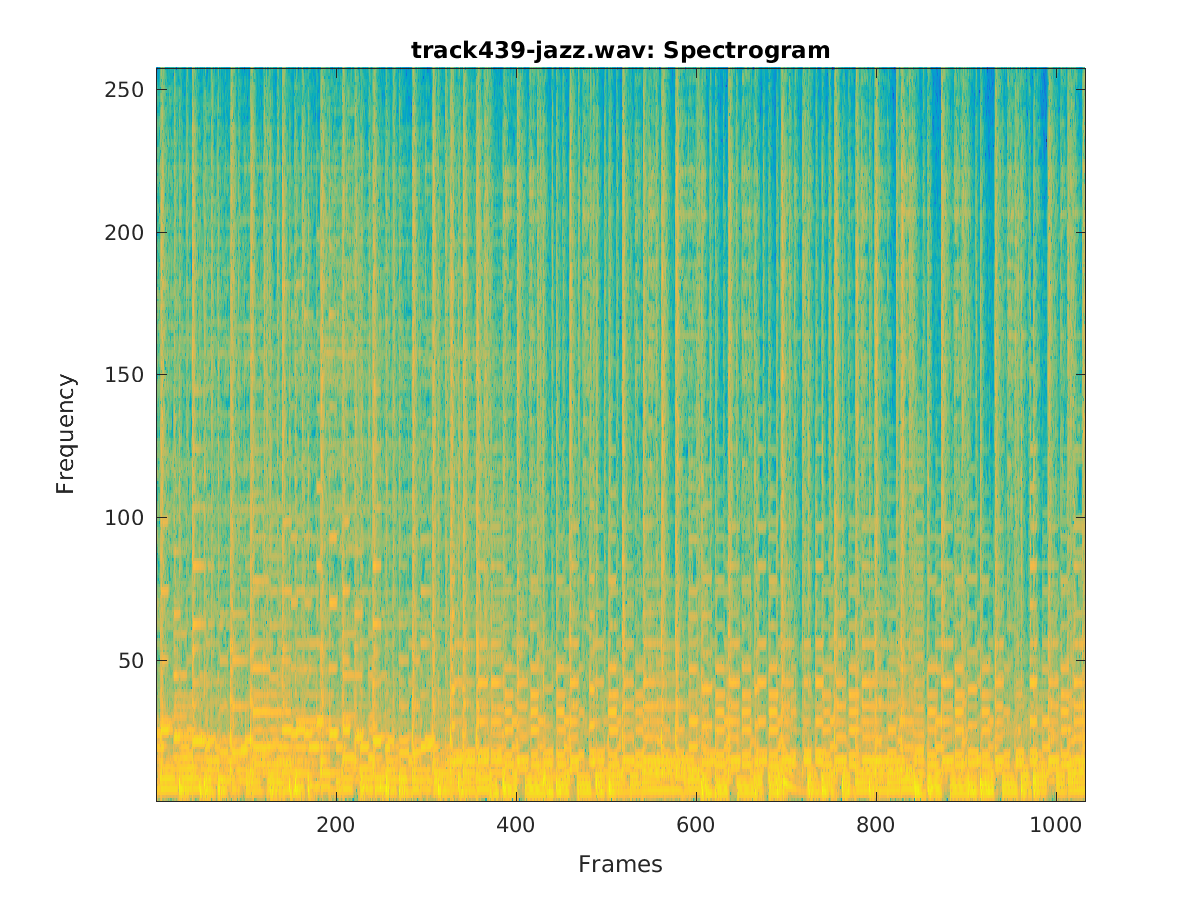
\includegraphics[width=.75\textwidth]{track439-jazz-specto.png}
    \caption{track437-jazz}
\end{figure}
\begin{figure}[H]
    \centering
    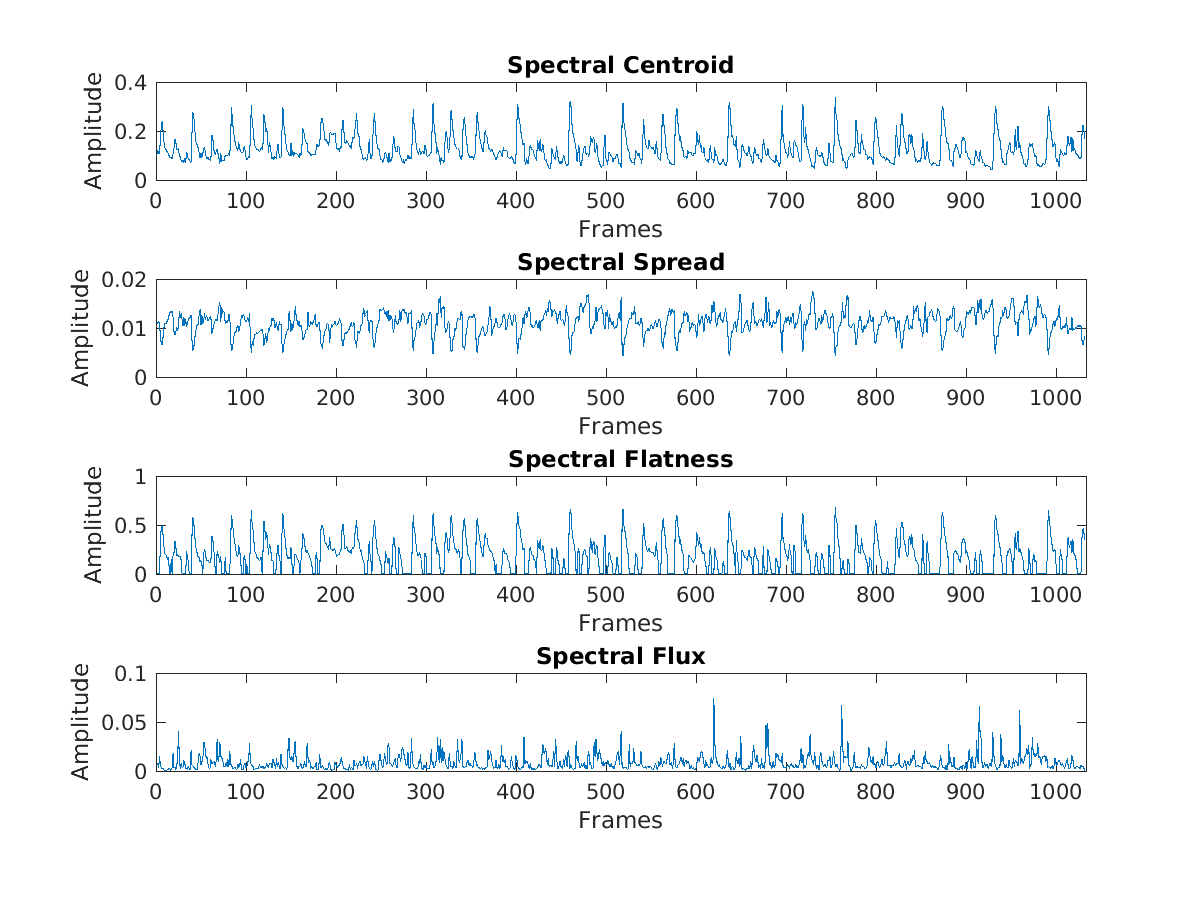
\includegraphics[width=1\textwidth]{track439-jazz-spectral.png}
    \caption{track437-jazz}
\end{figure}

\pagebreak

There are moments in the song, where the spectrogram is displaying a lot of power in all the frequency ranges. The exact instrument producing this spread of frequency is most likely from the drums. \\

The centroid has large spikes during the moments in the frame that has a large range of frequencies being played. Unlike the previous jazz track, this does not share that many characteristics, and it cannot be seen how they are from the same genre. \\

Flatness seem to directly correspond with the moments in the frames where there is a wide spectrum of frequencies being played. \\

The flux is mostly the same since there is not that many changes between the frames. Looking at the spectrogram after frames 250 actually seem to be oscillating between several frequencies. 

\pagebreak

\begin{figure}[H]
    \centering
    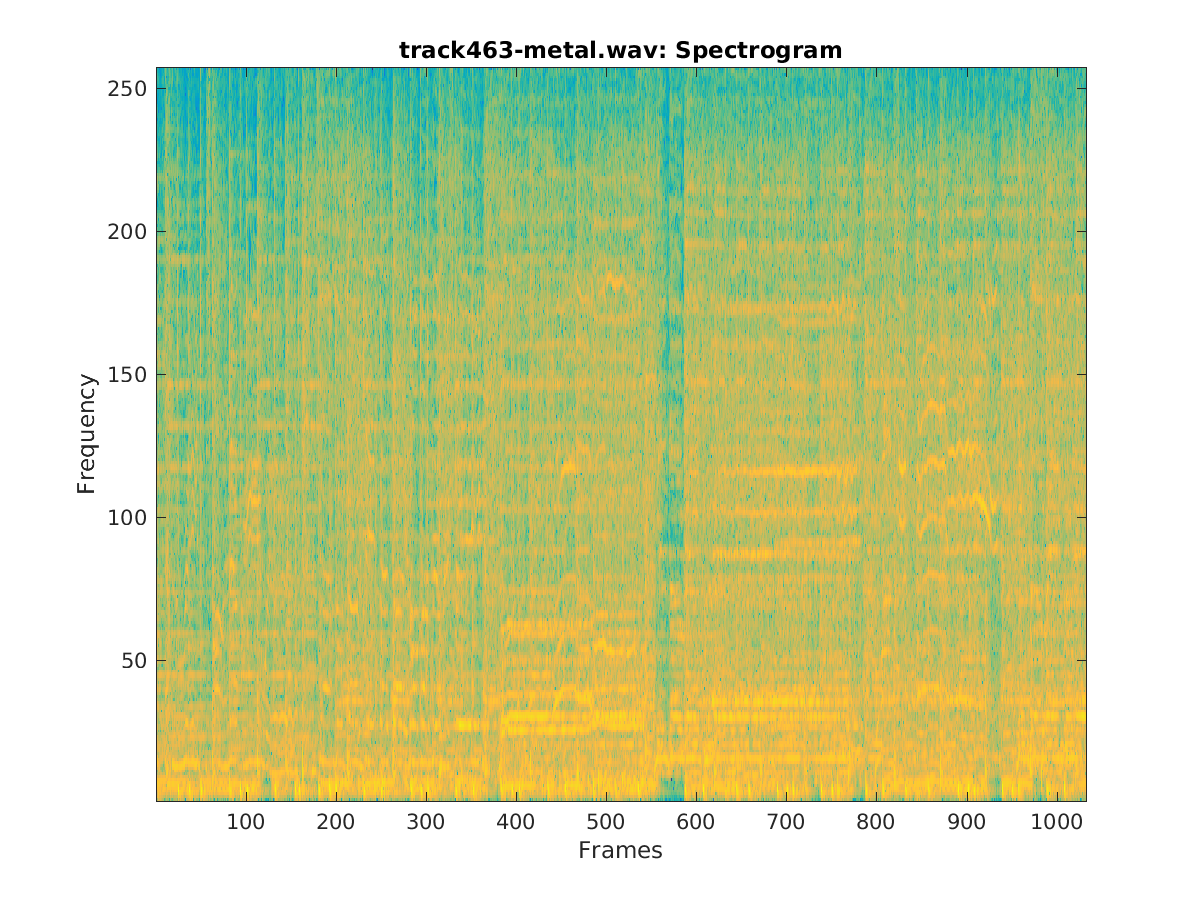
\includegraphics[width=.75\textwidth]{track463-metal-specto.png}
    \caption{track463-metal}
\end{figure}
\begin{figure}[H]
    \centering
    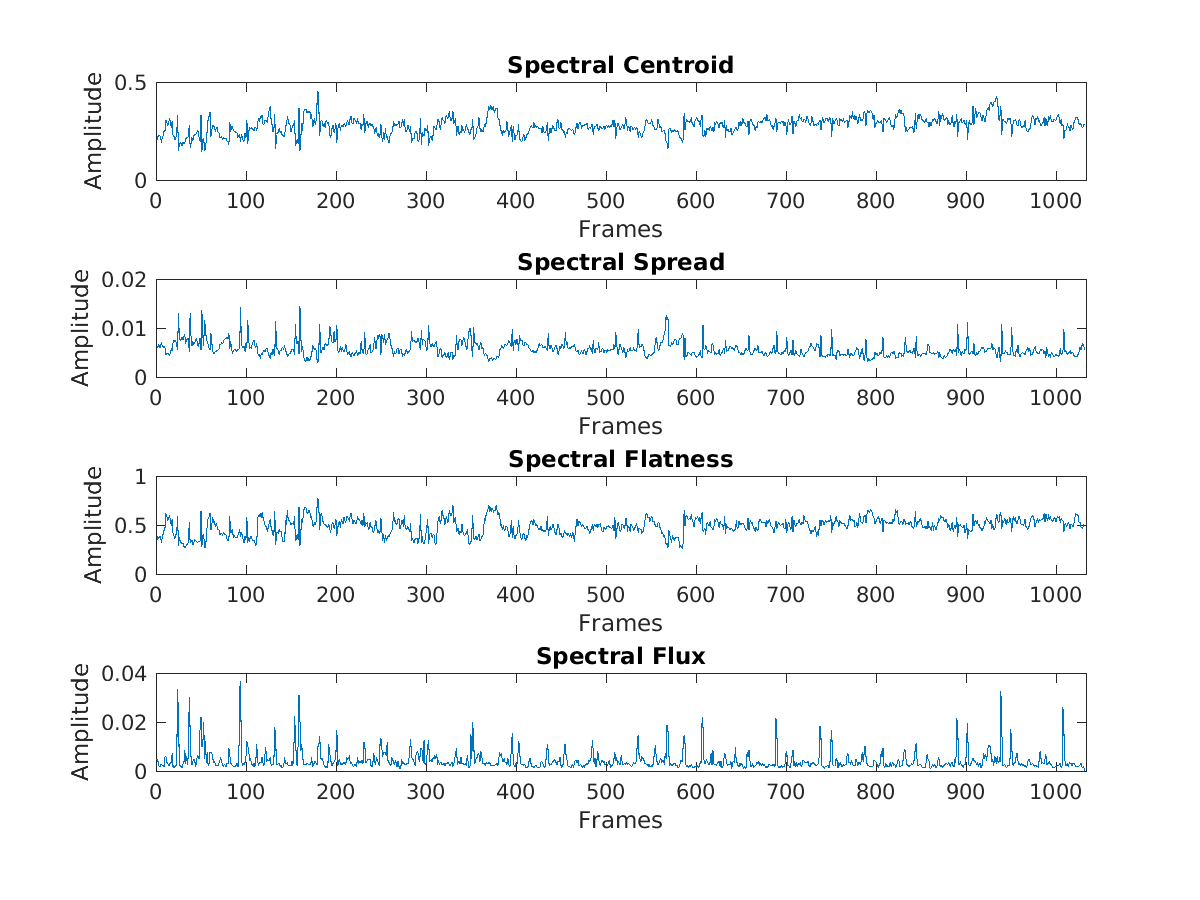
\includegraphics[width=1\textwidth]{track463-metal-spectral.png}
    \caption{track463-metal}
\end{figure}

\pagebreak
This song is very noisy and loud and causing the spectrogram to not give a lot of information. Its not easy at all to tell where the song is by looking and listening to the song. \\

It is hard to say what the significance of all three spectrum plots are in context of the spectrogram. It is hard to determine the correlation between all three. \\

\pagebreak
\begin{figure}[H]
    \centering
    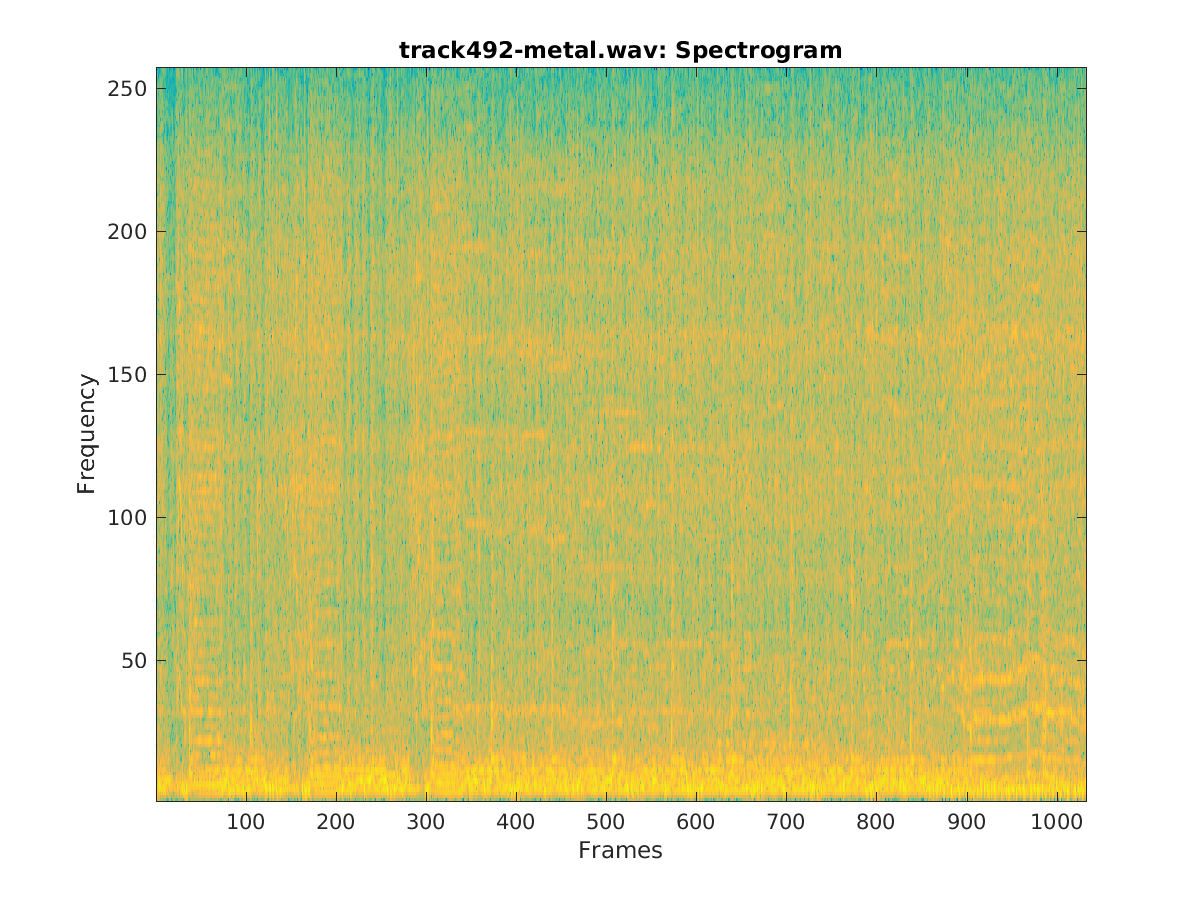
\includegraphics[width=.75\textwidth]{track492-metal-specto.png}
    \caption{track492-metal}
\end{figure}
\begin{figure}[H]
    \centering
    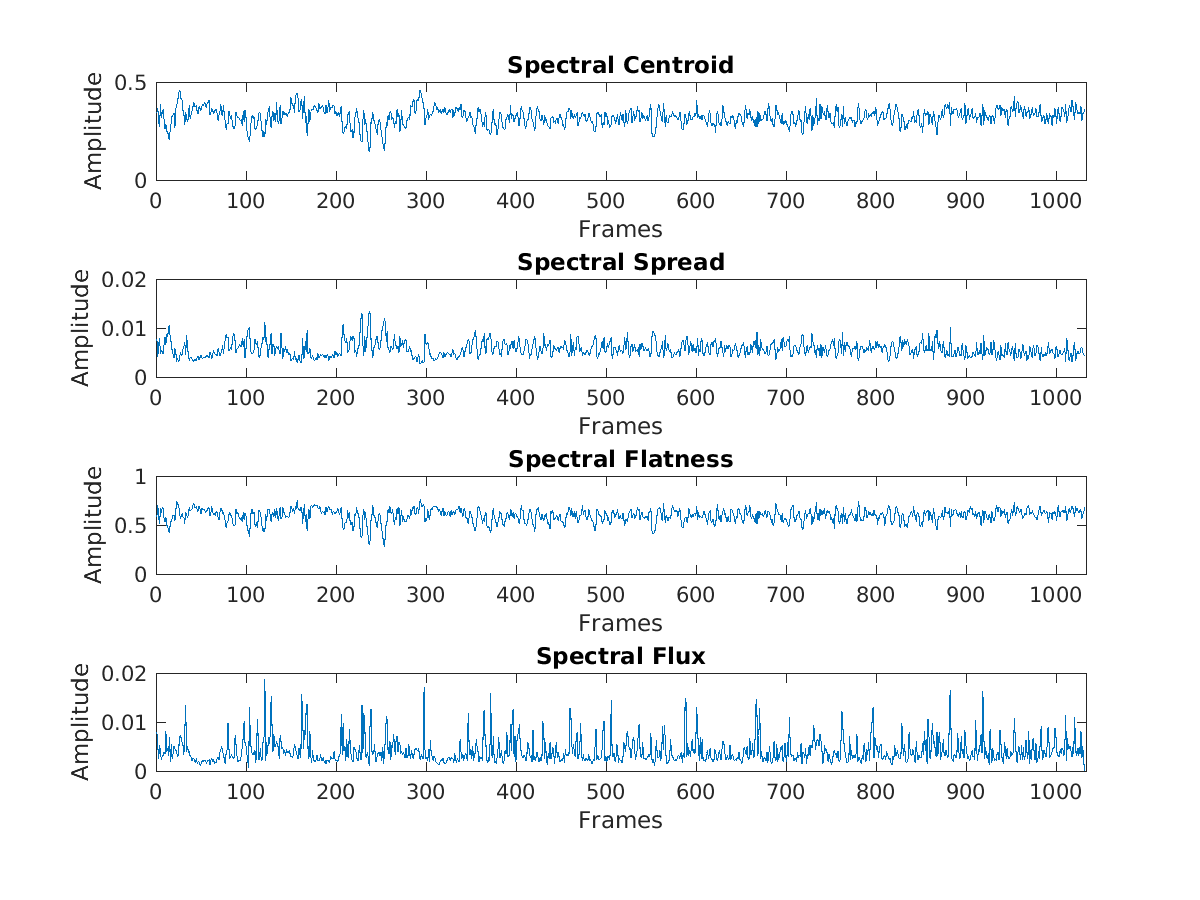
\includegraphics[width=1\textwidth]{track492-metal-spectral.png}
    \caption{track492-metal}
\end{figure}
\pagebreak

Like the previous metal track, this is extremely noisy of a track. There are some parts of the spectrogram that is recognized in the song, specifically the parts where they are quieter. \\
`
In the centroid and spread, there are obvious changes at frames 75, 200, and 300 that are shown, where the centroid and spread are increase and decreasing. It can be said from the flatness that the song is mostly noisy due to the magnitude of the song, as seen by the spectrum and the sound. \\

\pagebreak
\begin{figure}[H]
    \centering
    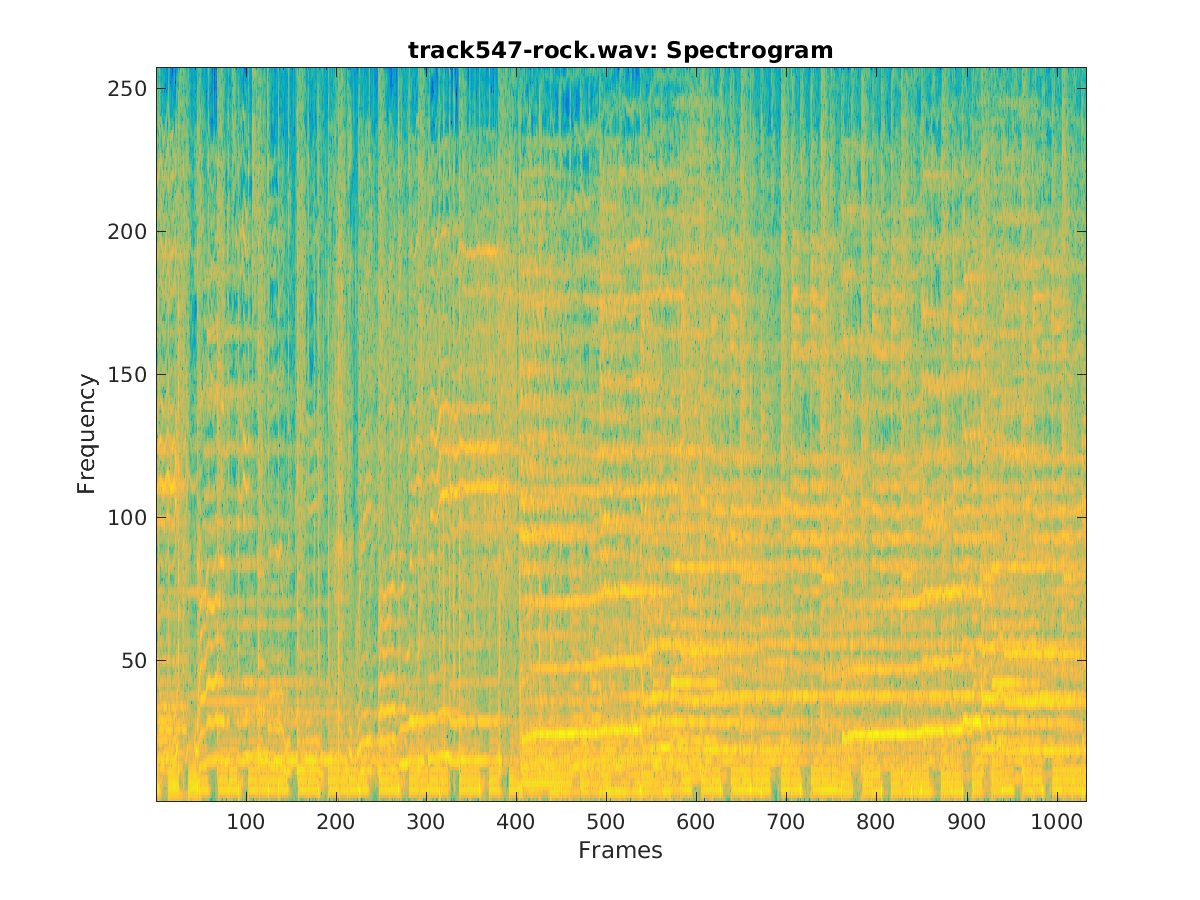
\includegraphics[width=.75\textwidth]{track547-rock-specto.png}
    \caption{track547-rock}
\end{figure}
\begin{figure}[H]
    \centering
    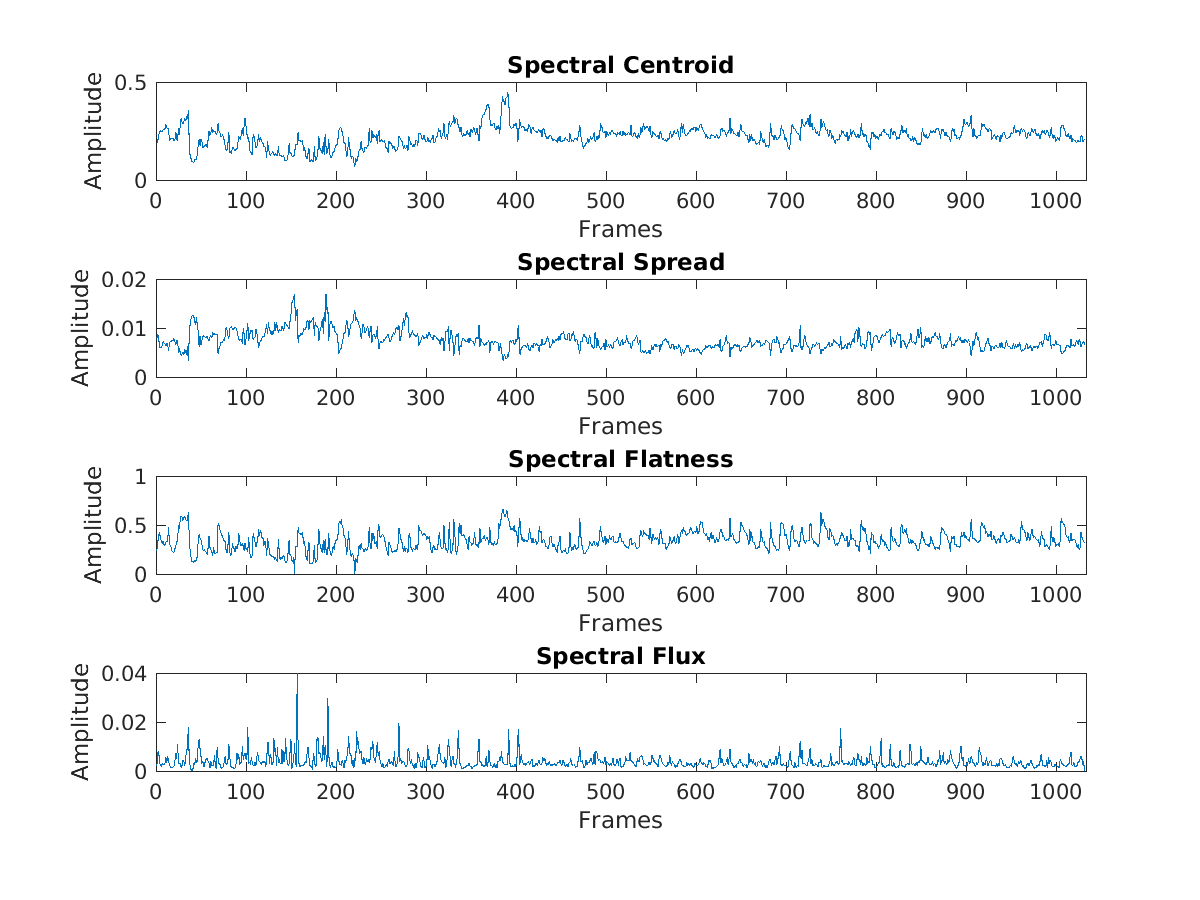
\includegraphics[width=1\textwidth]{track547-rock-spectral.png}
    \caption{track547-rock}
\end{figure}
\pagebreak 

The first rock track spectrogram is much easier to tell where the song is playing. The beat of the song is seen in the first 250 frames of the song, and as well as the sudden increase after. \\

There is an obvious shift at frame 400 when the song changes a bit and this is shown in centroid and spread. One important note is the similarities between rock and metal have. It may cause difficulties later to tell the difference between these two genres. \\

There is very low changes between the frames and thus the low flux values. 

\pagebreak
\begin{figure}[H]
    \centering
    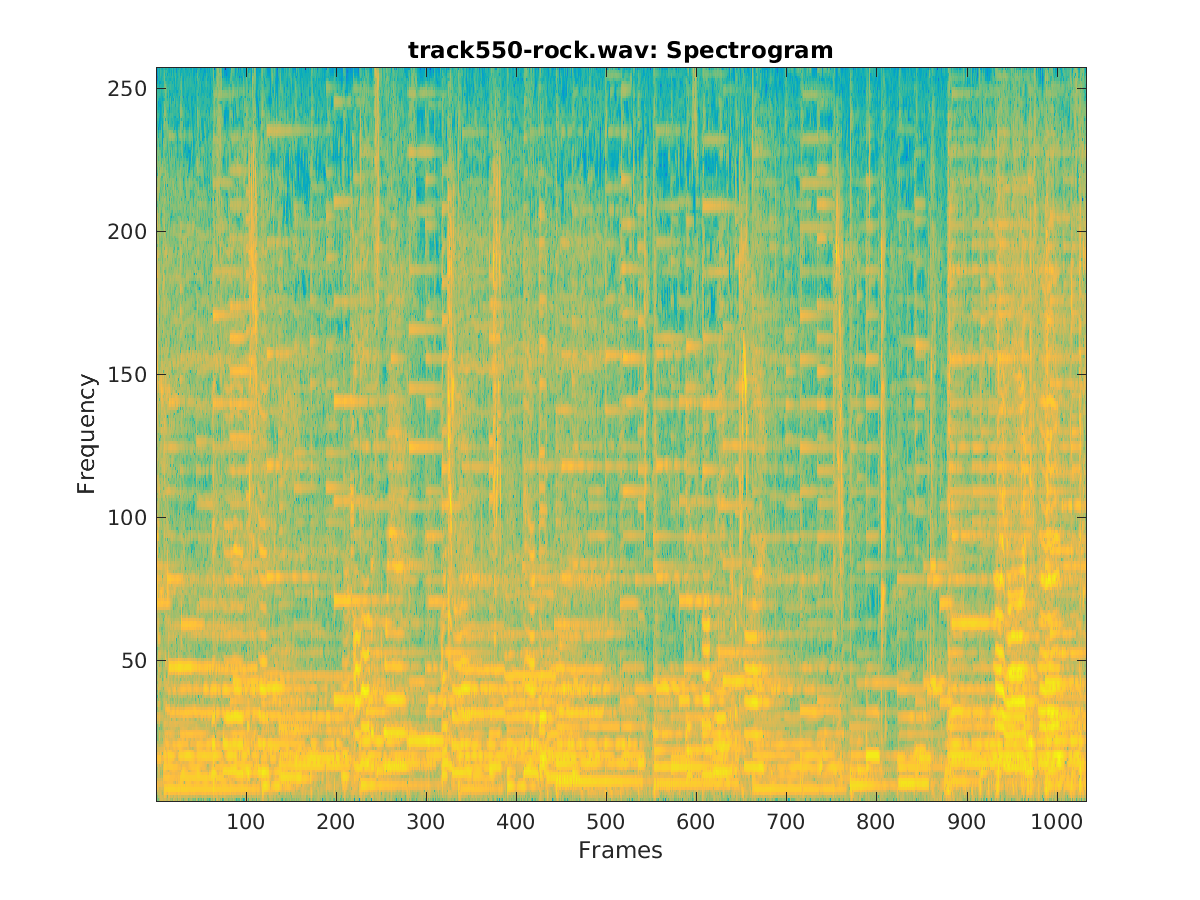
\includegraphics[width=.75\textwidth]{track550-rock-specto.png}
    \caption{track550-rock}
\end{figure}


\begin{figure}[H]
    \centering
    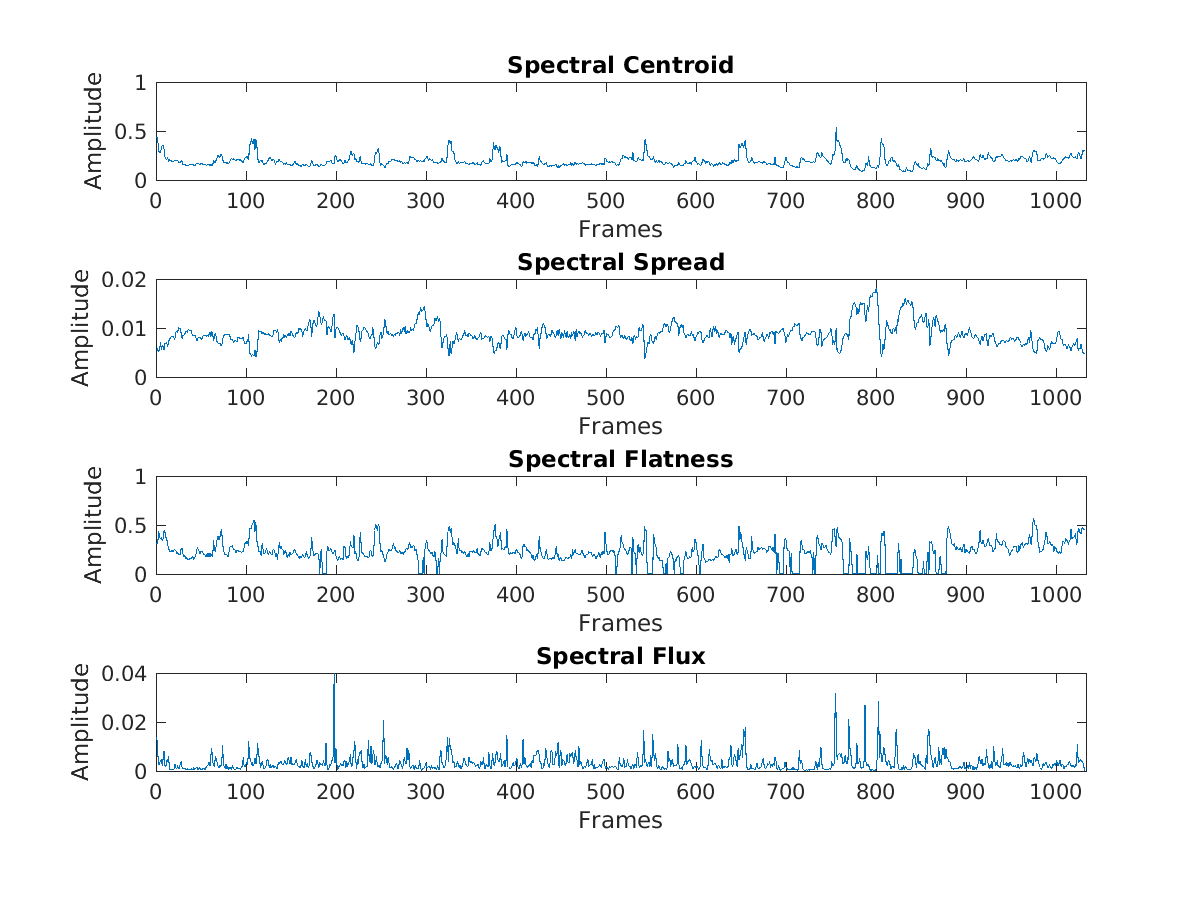
\includegraphics[width=\textwidth]{track550-rock-spectral.png}
    \caption{track550-rock}
\end{figure}
\pagebreak

This rock track does not seem to have a correlation between itself and the spectrogram. \\

The centroid does not change for the most part throughout the song, and as seen in the spectrogram, the frequencies being played do no change that often. This is reflected in the flux as well, since for most of the song, the flux is mostly zero. \\


\pagebreak
\begin{figure}[H]
    \centering
    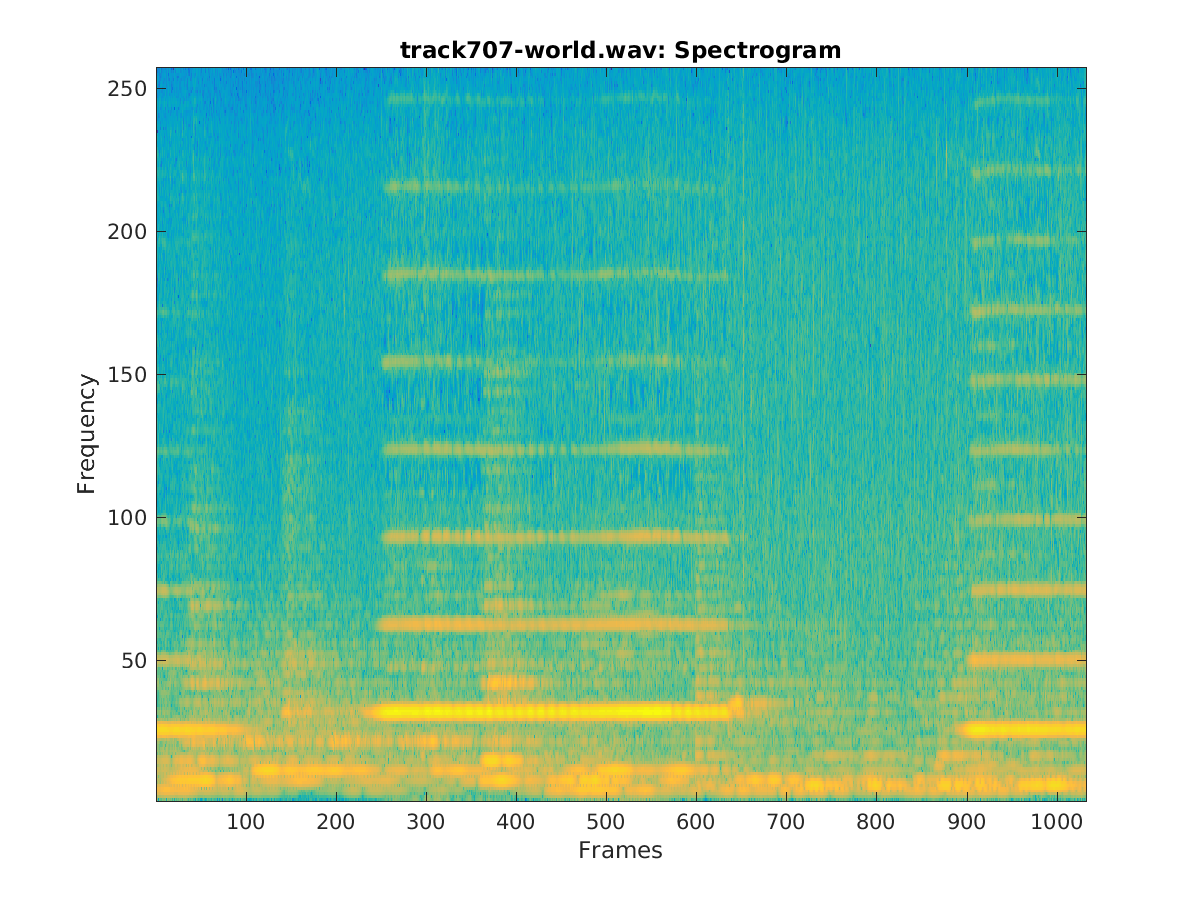
\includegraphics[width=.75\textwidth]{track707-world-specto.png}
    \caption{track707-world}
\end{figure}
\begin{figure}[H]
    \centering
    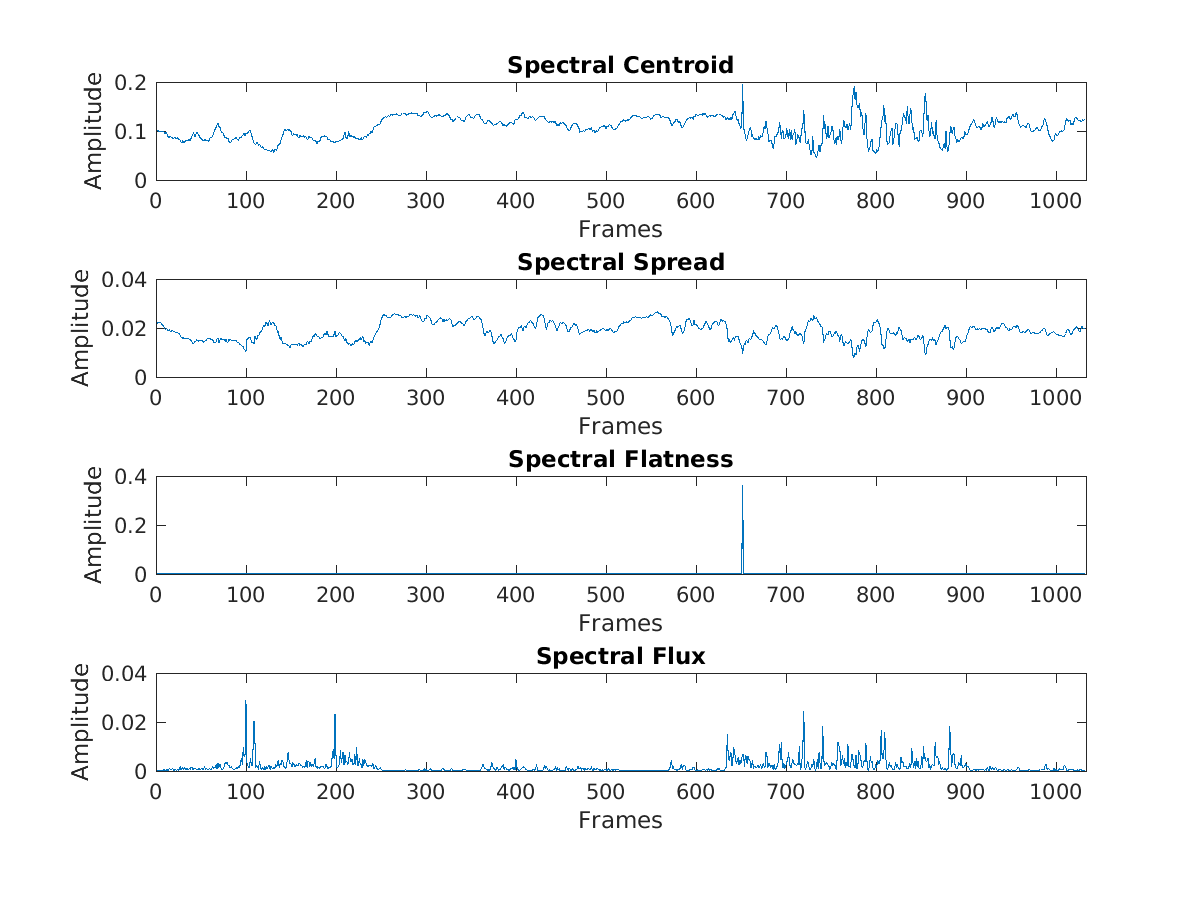
\includegraphics[width=1\textwidth]{track707-world-spectral.png}
    \caption{track707-world}
\end{figure}
\pagebreak

In this world track, there is evidence of a pure tone being played after the 250th frame. This sudden increase in power of the frequency bands, especially at a specific one demonstrates there is a pure sine wave being played of some sorts. \\

The centroid and spread do not seem to have much valuable information when analyzing the track. It is more valuable to look at the actual spectrogram to gain information on the spread of the frequencies and the center one. \\

The flatness is mostly zero except fro when the song goes quiet from the noise produced. \\

The flux is mostly zero when the noise is produced. 
\pagebreak
\begin{figure}[H]
    \centering
    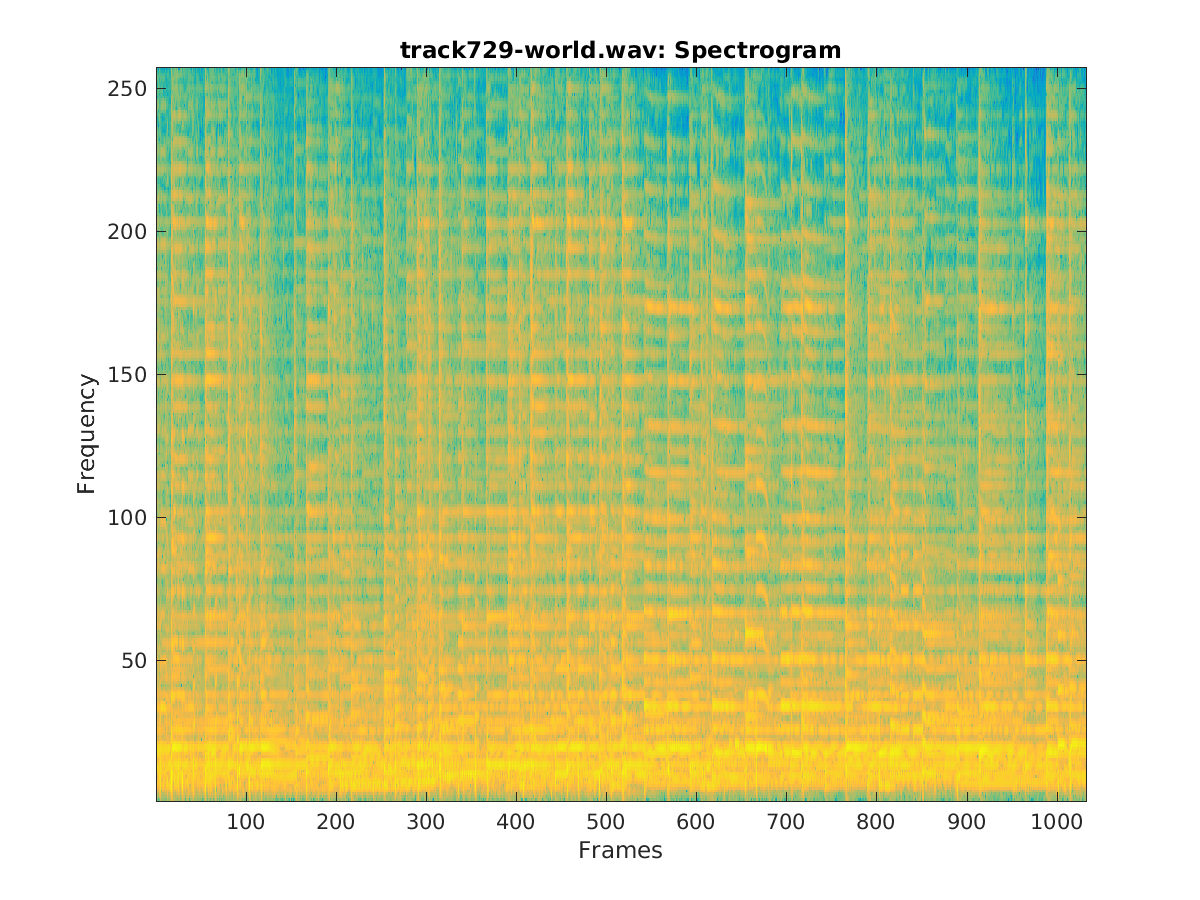
\includegraphics[width=.75\textwidth]{track729-world-specto.png}
    \caption{track729-world}
\end{figure}
\begin{figure}[H]
    \centering
    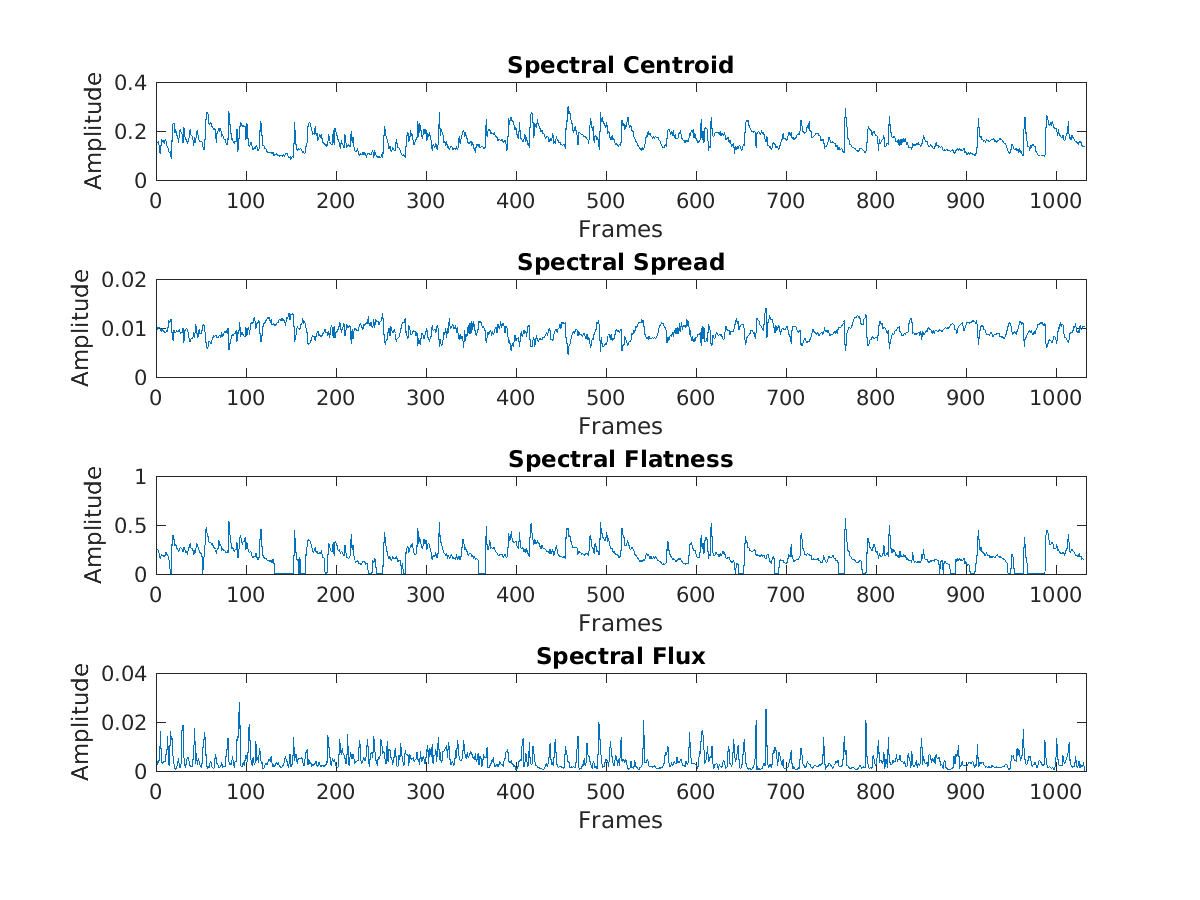
\includegraphics[width=1\textwidth]{track729-world-spectral.png}
    \caption{track729-world}
\end{figure}
\pagebreak
The strumming of the guitar can be seen in the spectrogram, but other than that, it is hard to tell of any other type of noise being played. \\

The spread and centroid seen several spikes at certain frames as seen in the spectrogram, but there are other spikes that would be expected to be seen. \\

The flatness fluctuates a lot as demonstrate the sudden plucking of the guitars and causing the flatness to increase dramatically. \\

The flux is changing a lot from frame to frame. 

\subsection{Conclusion: Spectral Analysis}

The spectrogram mostly shows the main frequency components that are being played, but it is obvious that the signal, without being filtered, is going to produce a lot of useless or repetitive information. For a majority of the spectrogram, the low frequencies were the main content of the spectrum. \\

The centroid and spread demonstrates useful information that gives a concise set of data that shows how each frame has a main frequency, and the spread of frequency between the other frequency bands. For the most part, however, it gives characteristics of the song, but not the genre specifically. This idea of genre classification gives difficulty to figuring out what the meaning of the centroid and spread mean. \\

The flatness also seems not very useful in genre classification. It is simply another measure of the song characteristics. \\

The flux demonstrates the changes between frequency content in bands and this may be a more meaningful information because genres may have a way of changing notes in a song in a more dramatic, or calm manner. \\ 

Overall, these spectrum tools are useful to give a better analysis to the song, but not necessarily to the genre. 

\section{MFCC Coefficients}

\subsection{Filter Banks}

\lstinputlisting[language=Matlab]{../fbanks.m}

\begin{figure}[H]
    \centering
    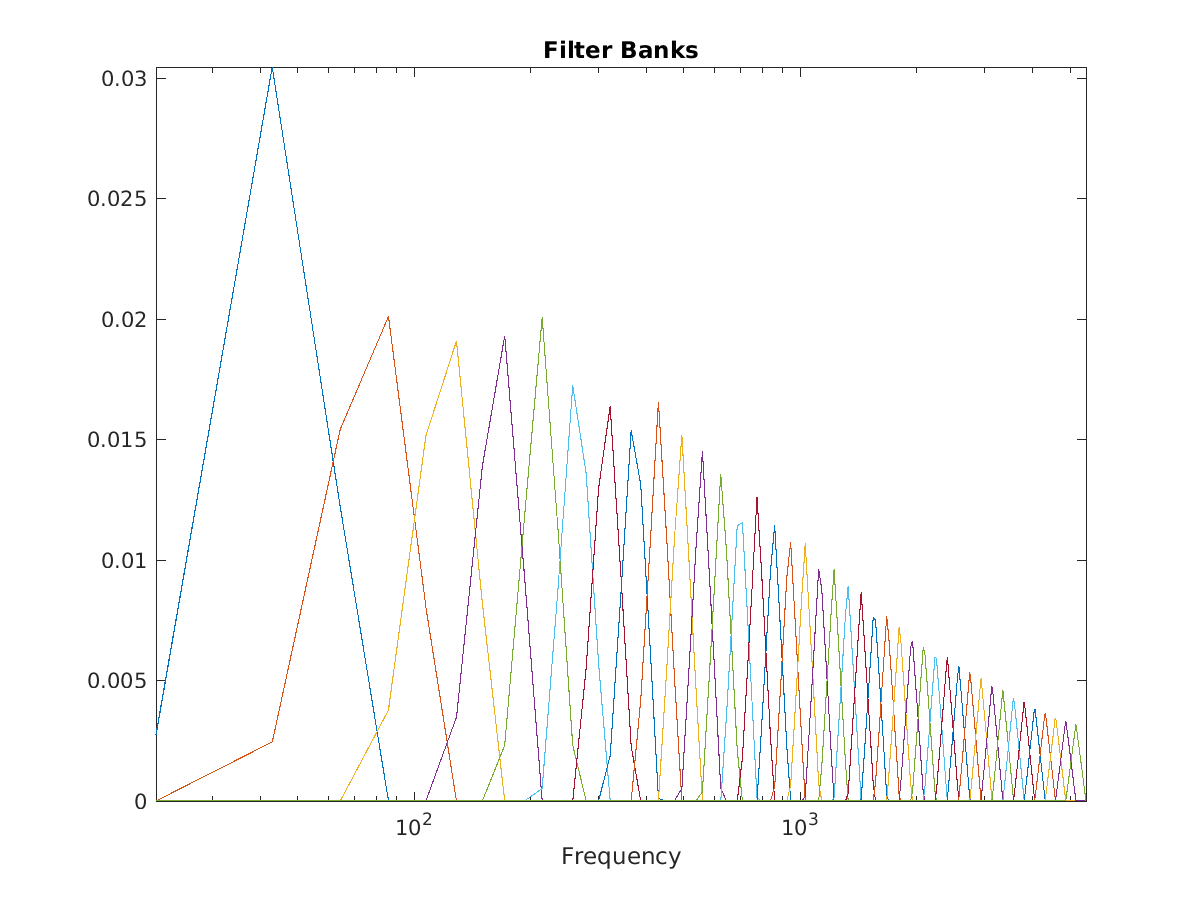
\includegraphics[width=.8\textwidth]{filterbanks.png}
    \caption{Filter Banks}
\end{figure}

\subsection{MFCC Graphs}

Without going into too much detail on each individual track, when looking at all the MFCC coefficient graphs and comparing them to the spectrogram, there is a lot more detail that can be seen. The notes being played at certain times is a lot more obvious and it is not as noisy as before. This collection of information that describe the frequency spectrum content of each song is a little more useful than the time domain material, but it does not mean that this dictates genre. Some genre may or may not have the same frequency ranges it utilizes, but it definitely has more power and information than time.


\lstinputlisting[language=Matlab]{../mfcc.m}

\begin{figure}[H]
    \centering
    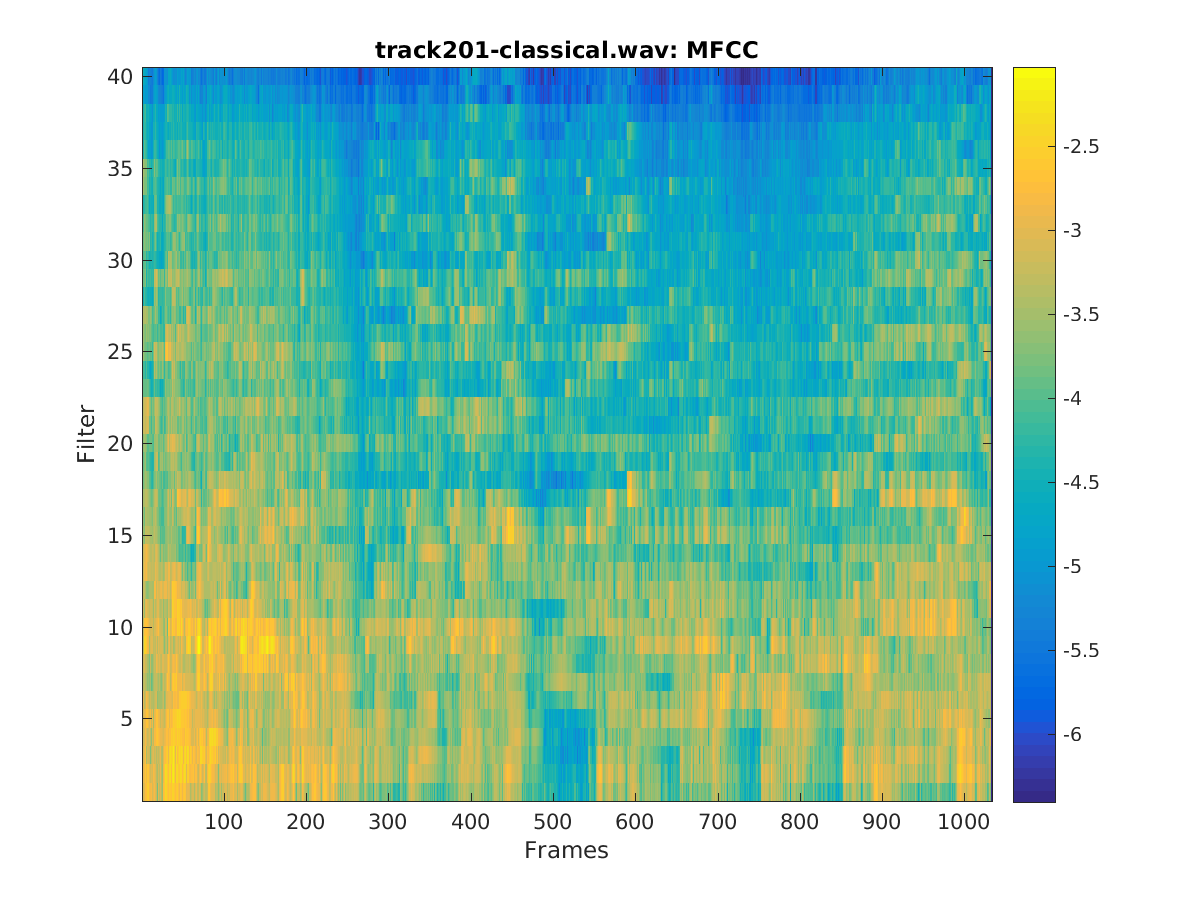
\includegraphics[width=.8\textwidth]{track201-classical-mfcc.png}
    \caption{track201-classical}
\end{figure}


\begin{figure}[H]
    \centering
    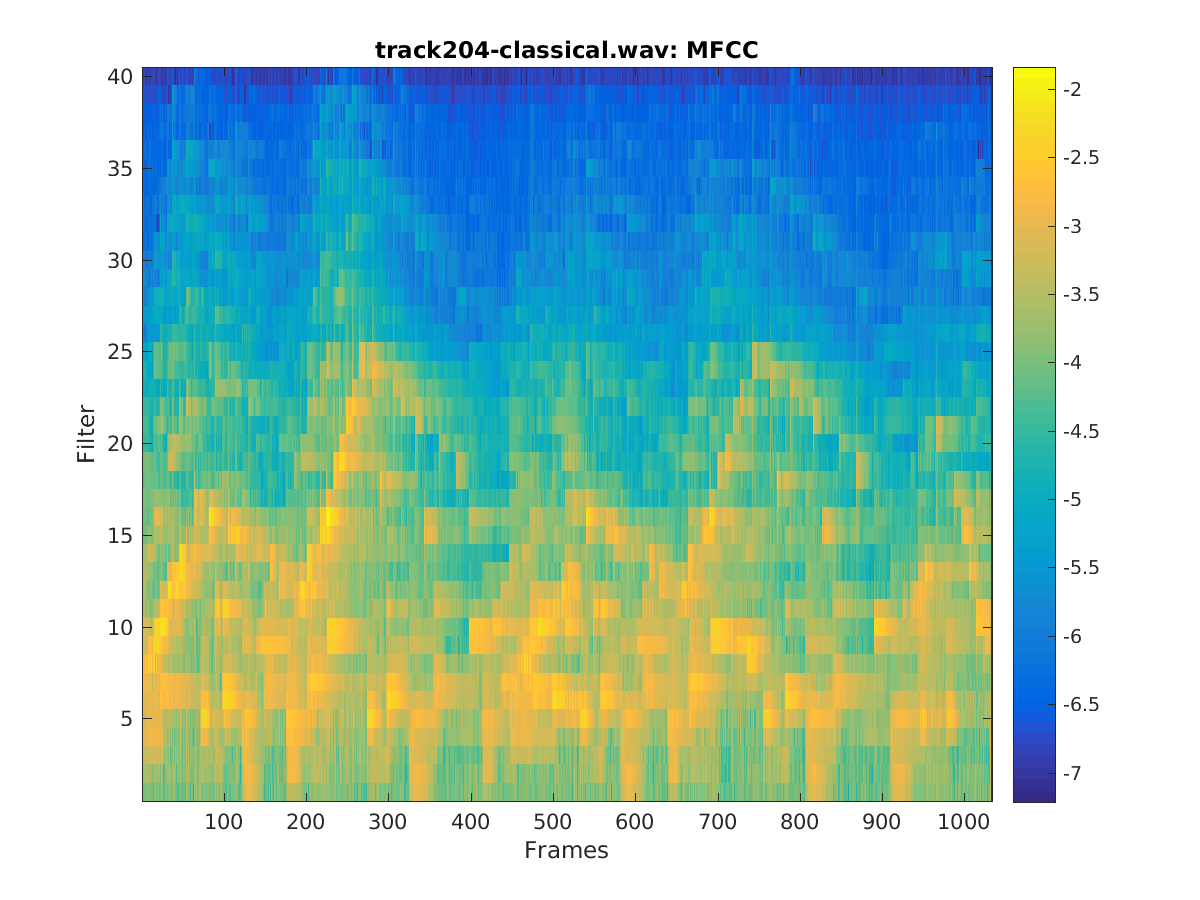
\includegraphics[width=.8\textwidth]{track204-classical-mfcc.png}
    \caption{track204-classical}
\end{figure}


\begin{figure}[H]
    \centering
    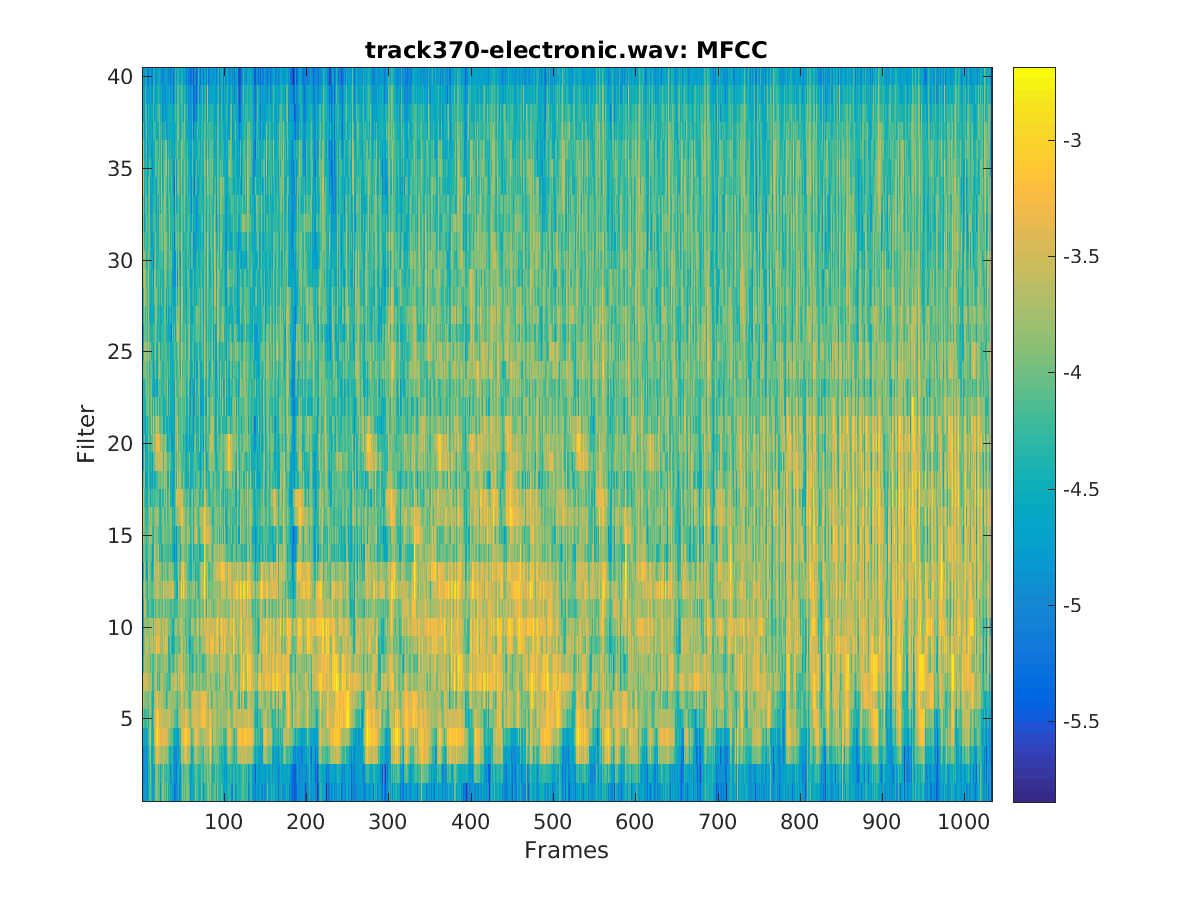
\includegraphics[width=.8\textwidth]{track370-electronic-mfcc.png}
    \caption{track370-electronic}
\end{figure}


\begin{figure}[H]
    \centering
    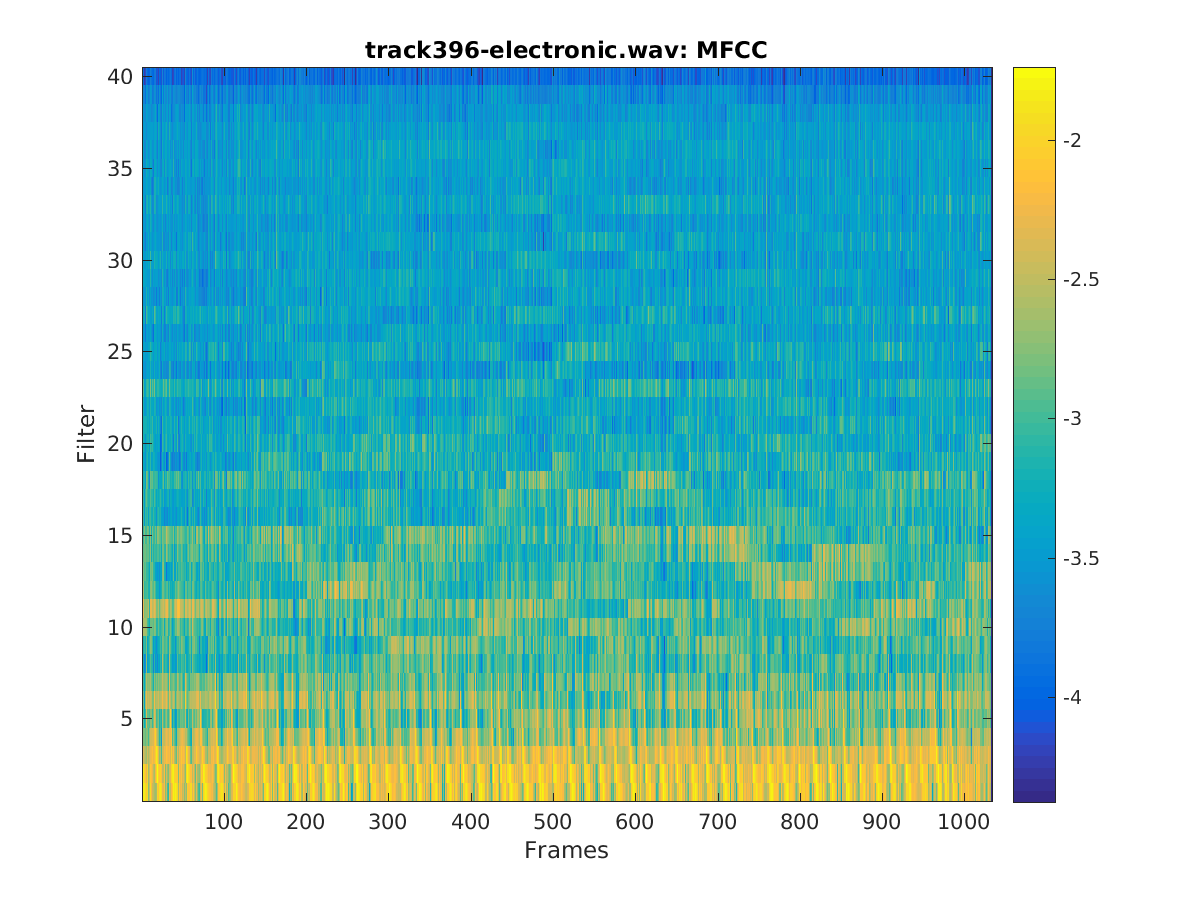
\includegraphics[width=.8\textwidth]{track396-electronic-mfcc.png}
    \caption{track396-electronic}
\end{figure}


\begin{figure}[H]
    \centering
    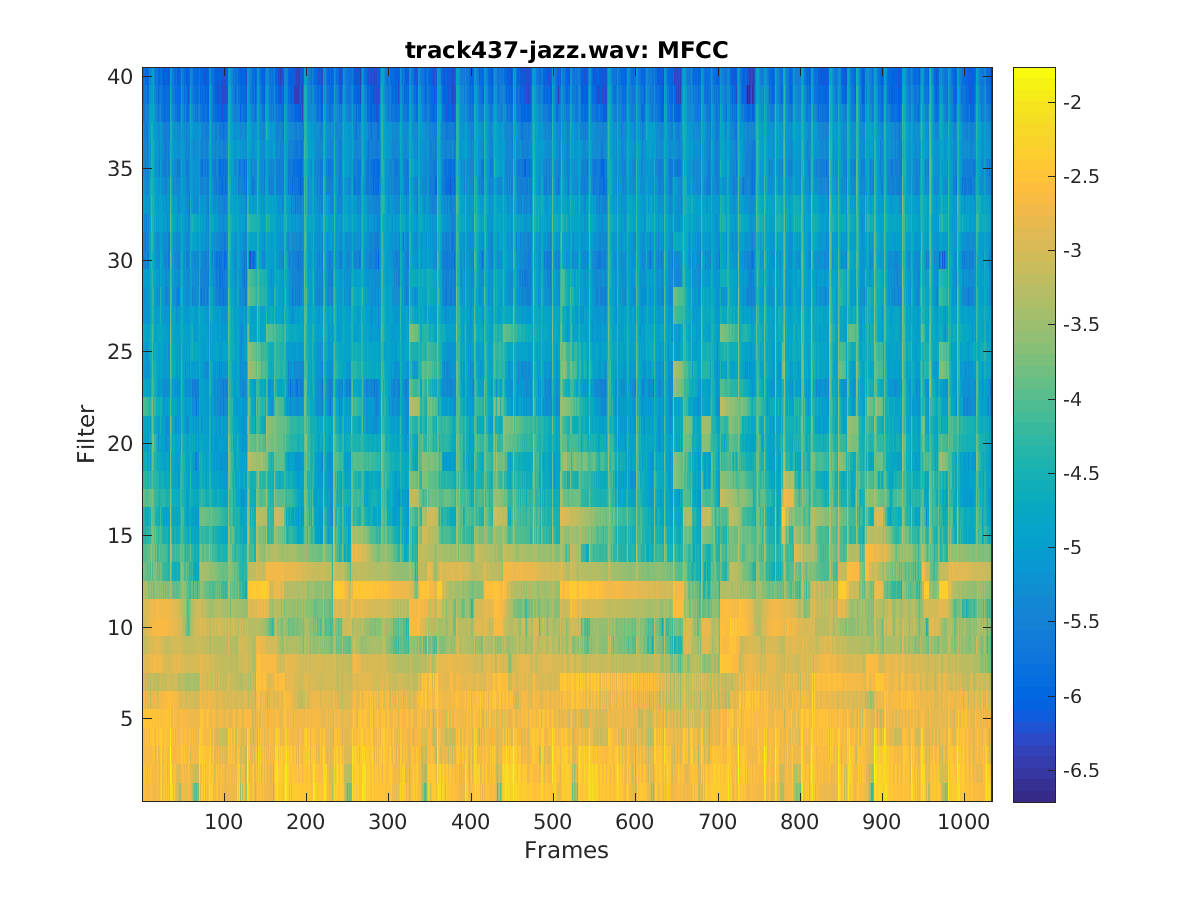
\includegraphics[width=.8\textwidth]{track437-jazz-mfcc.png}
    \caption{track437-jazz}
\end{figure}


\begin{figure}[H]
    \centering
    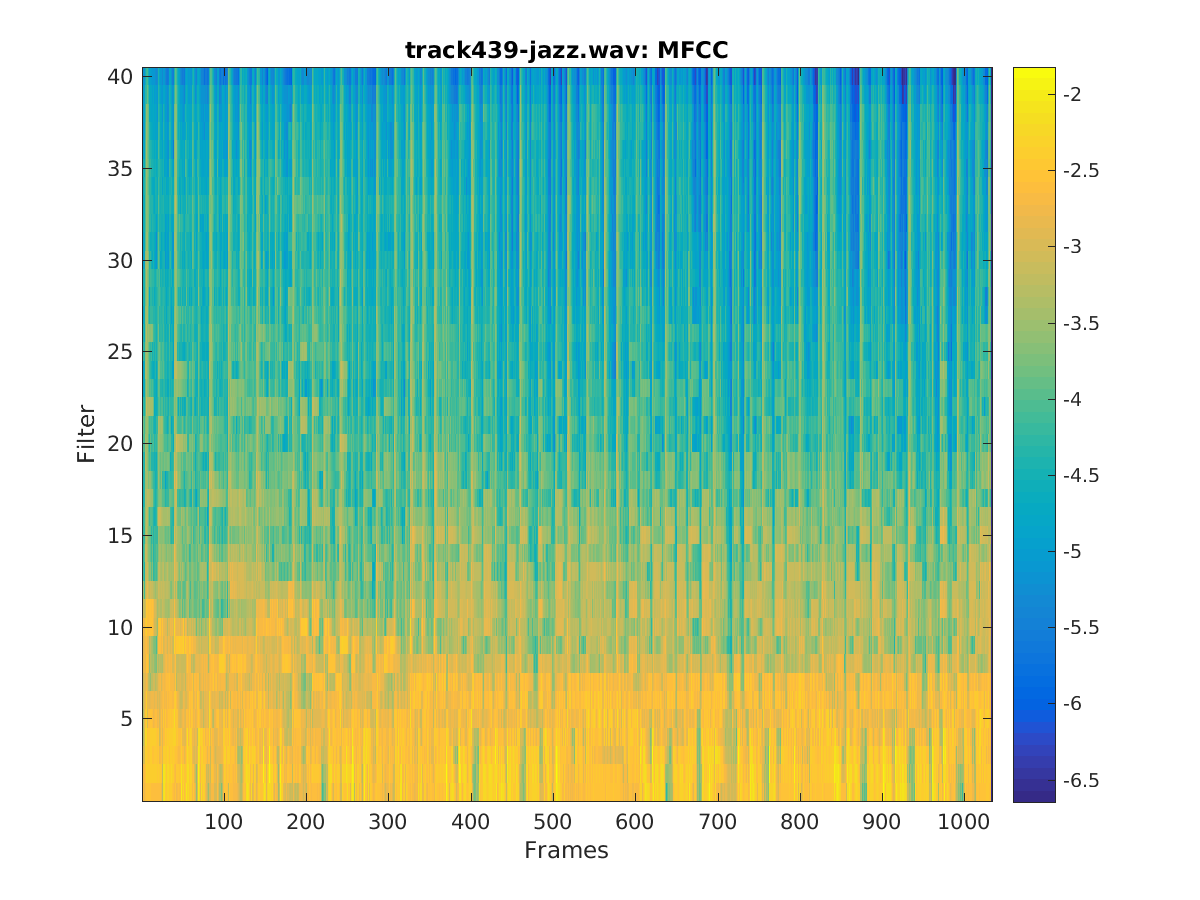
\includegraphics[width=.8\textwidth]{track439-jazz-mfcc.png}
    \caption{track437-jazz}
\end{figure}


\begin{figure}[H]
    \centering
    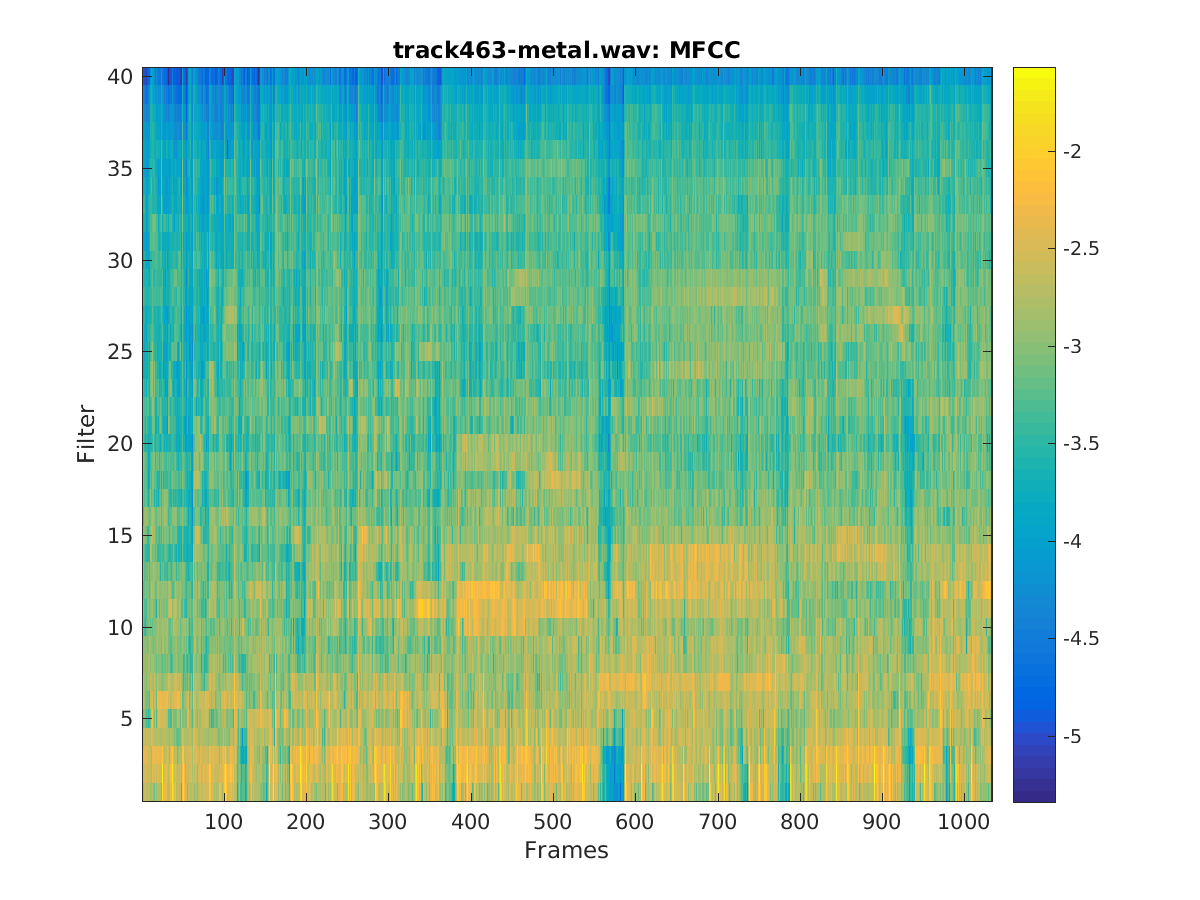
\includegraphics[width=.8\textwidth]{track463-metal-mfcc.png}
    \caption{track463-metal}
\end{figure}

\begin{figure}[H]
    \centering
    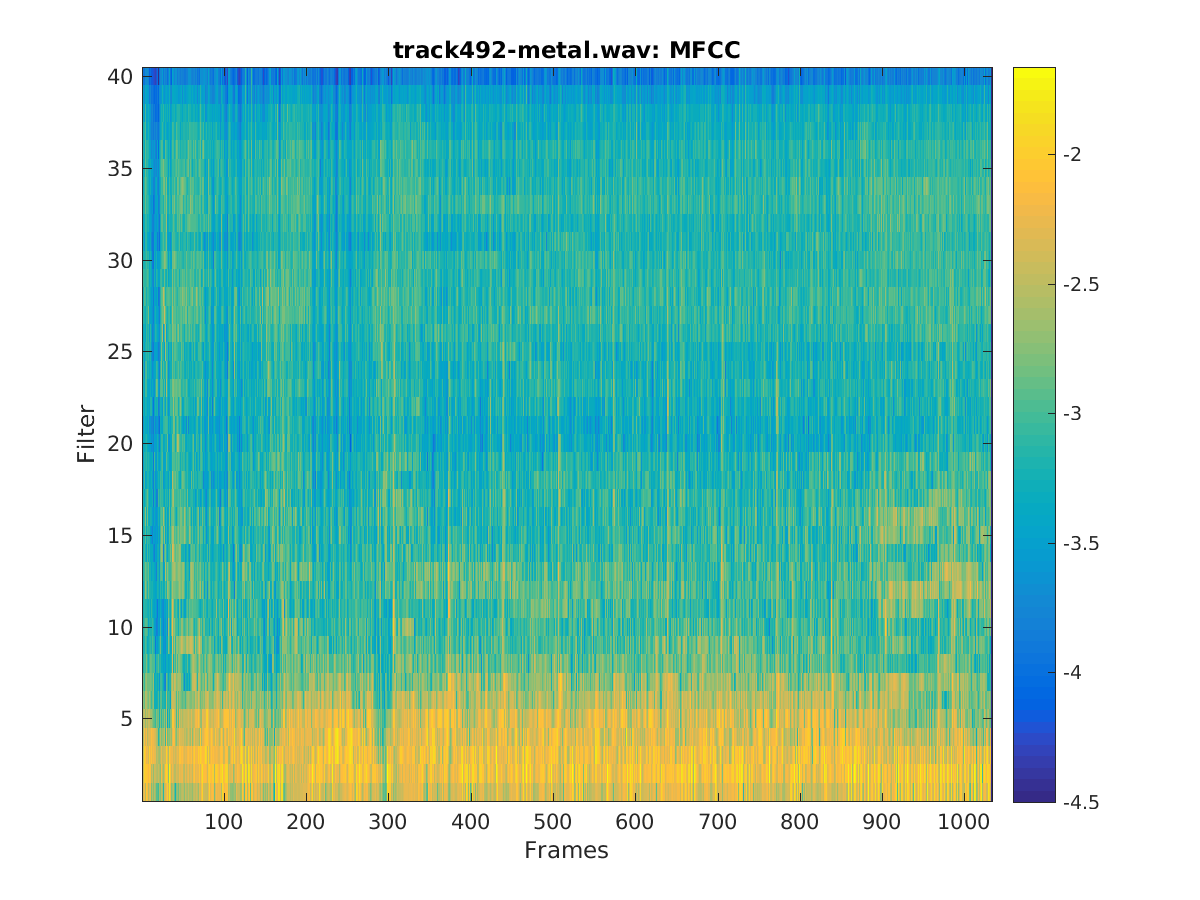
\includegraphics[width=.8\textwidth]{track492-metal-mfcc.png}
    \caption{track492-metal}
\end{figure}


\begin{figure}[H]
    \centering
    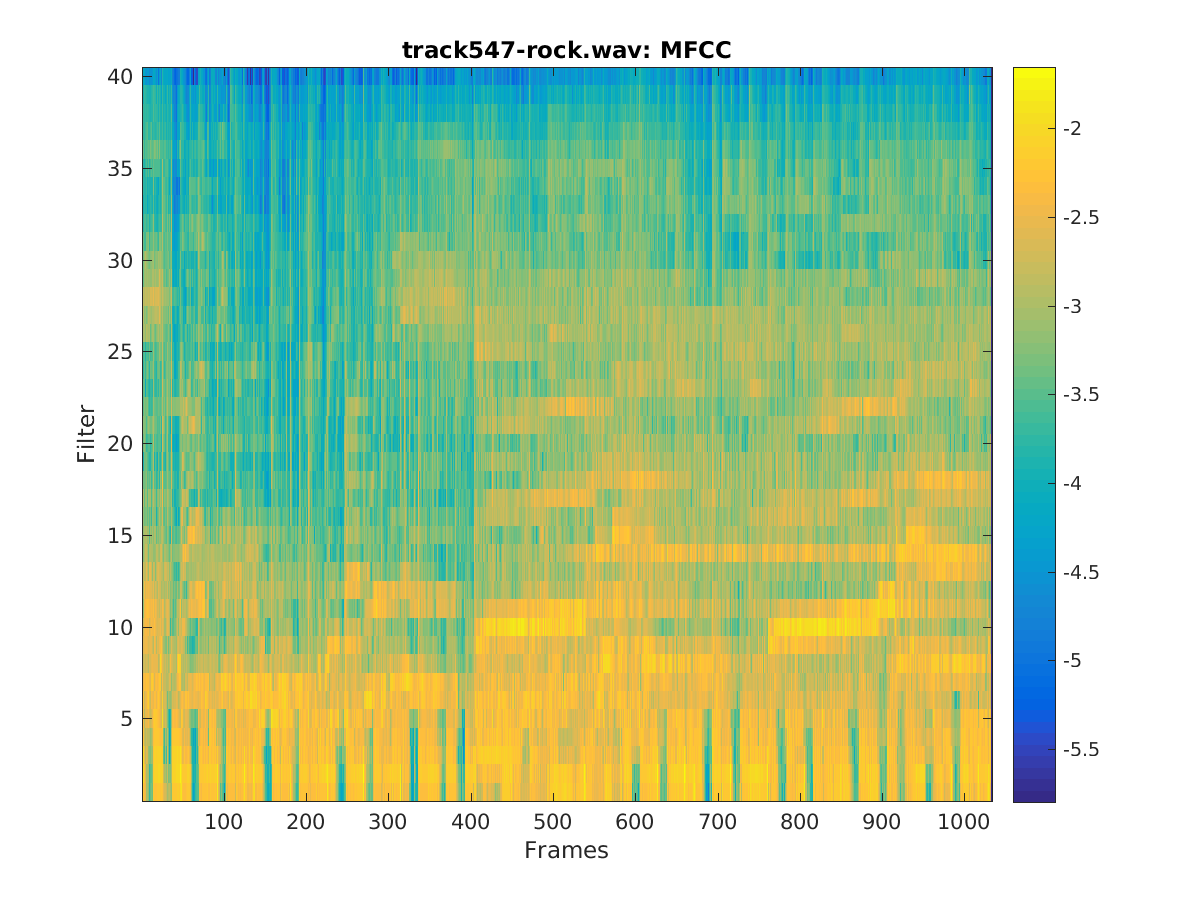
\includegraphics[width=.8\textwidth]{track547-rock-mfcc.png}
    \caption{track547-rock}
\end{figure}


\begin{figure}[H]
    \centering
    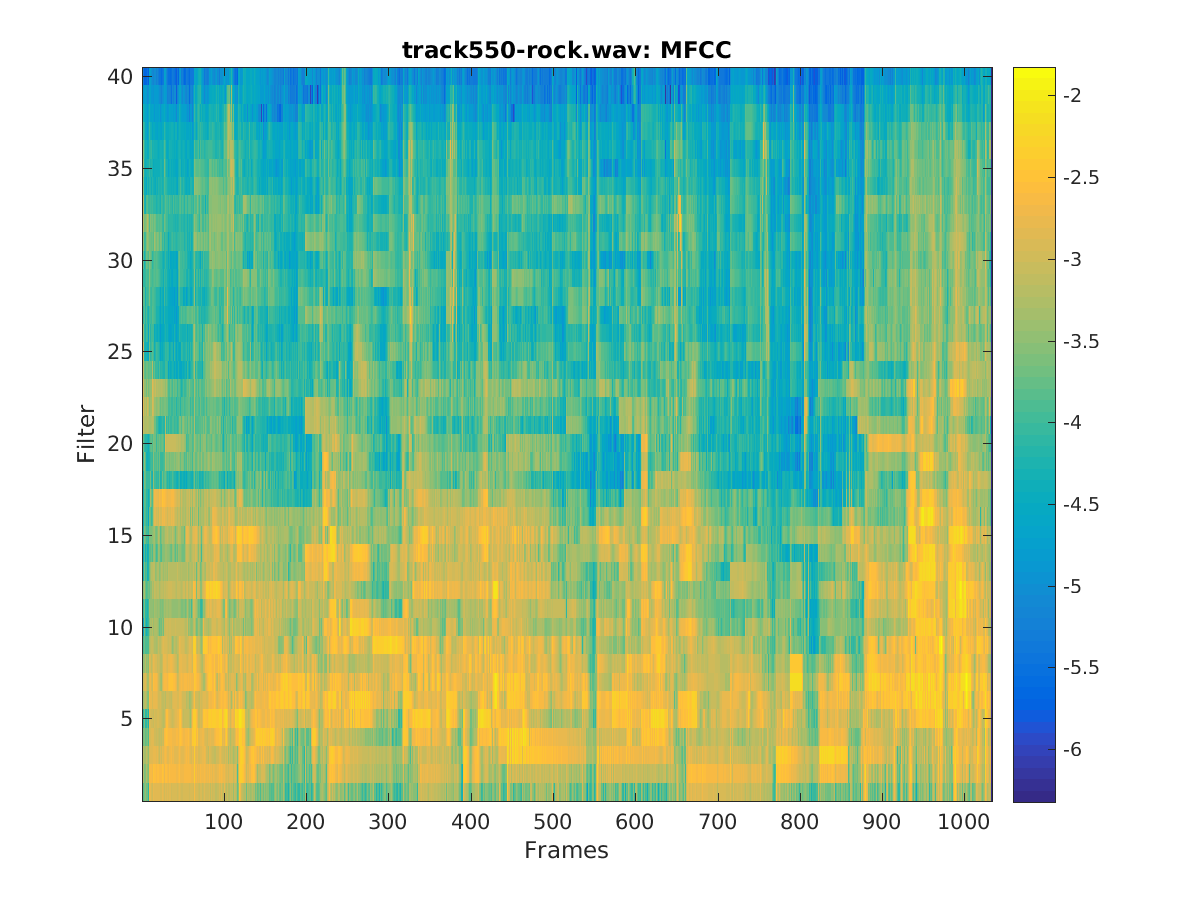
\includegraphics[width=.8\textwidth]{track550-rock-mfcc.png}
    \caption{track550-rock}
\end{figure}


\begin{figure}[H]
    \centering
    \includegraphics[width=.8\textwidth]{track707-world-mfcc.png}
    \caption{track707-world}
\end{figure}


\begin{figure}[H]
    \centering
    \includegraphics[width=.8\textwidth]{track729-world-mfcc.png}
    \caption{track729-world}
\end{figure}

\section{Conclusion}

Overall, the time domain material gives not so meaningful information on analyzing different genres. It simply refocused information that the original track shows. The spectral analysis, however, gave a broader set of information on the different type of frequency contents that the song gives, but it still struggles to seem to have any concrete information on what type of genre classification can look at. Finally, the MFCC give a stronger clue to what each song gives. These filtered signals are significantly cleaner and are visually more comprehensible unlike the spectrograms.

\appendix

\section{Code}

\subsection{Workspace Script}
\lstinputlisting[language=Matlab]{../workspace.m}

\subsection{Save Image Function}
\lstinputlisting[language=Matlab]{../saveImage.m}

\end{document}